\documentclass[notheorems,compress,mathserif,table]{beamer}

\useoutertheme{tree}
\usecolortheme{whale}      % Outer color themes, 其他选择: whale, seahorse, dolphin . 换一个编译看看有什么不同.
\usecolortheme{orchid}     % Inner color themes, 其他选择: lily, orchid
\useinnertheme[shadow]{rounded} % 对 box 的设置: 圆角、有阴影.
\setbeamercolor{sidebar}{bg=blue!50} % sidebar的颜色, 50%的蓝色.
%\setbeamercolor{background canvas}{bg=blue!9} % 背景色, 9%的蓝色. 去掉下一行, 试一试这个.
\setbeamertemplate{background canvas}[vertical shading][bottom=white,top=structure.fg!25] %%背景色, 上25%的蓝, 过渡到下白.
\usefonttheme{serif}  % 字体. 个人偏好有轮廓的字体. 去掉这个设置编译, 就看到不同了.
\setbeamertemplate{navigation symbols}{}   %% 去掉页面下方默认的导航条.
%%------------------------常用宏包---------------------------------------------------------------------
%%注意, beamer 会默认使用下列宏包: amsthm, graphicx, hyperref, color, xcolor, 等等
%\usepackage{CJK}
\usepackage{ctex}
\usepackage{amsmath,amsthm,amsfonts,amssymb,bm}
\usepackage{mathrsfs}
\usepackage{subfigure} %%图形或表格并排排列
\usepackage{xmpmulti}  %%支持文中的 \multiinclude 等命令, 使 mp 文件逐帧出现. 具体讨论见 beamer 手册.
\usepackage{colortbl,dcolumn}     %% 彩色表格
%\logo{
\includegraphics[height=0.09\textwidth]{ajln.jpg}}   %左上角科大logo
%%%%%%%%%%%%%%%%%%%%%%%%%%%%%%%%%%%%%%重定义字体、字号命令 %%%%%%%%%%%%%%%%%%%%%%%%%%%%%%%%%%%%%%%%%%%%%%
%\newcommand{\songti}{\CJKfamily{song}}        % 宋体
%\newcommand{\fangsong}{\CJKfamily{fs}}        % 仿宋体
%\newcommand{\kaishu}{\CJKfamily{kai}}         % 楷体
%\newcommand{\heiti}{\CJKfamily{hei}}          % 黑体
%\newcommand{\lishu}{\CJKfamily{li}}           % 隶书
\newcommand{\youyuang}{\CJKfamily{you}}       % 幼圆
\newcommand{\sanhao}{\fontsize{16pt}{\baselineskip}\selectfont}     % 字号设置
\newcommand{\sihao}{\fontsize{14pt}{\baselineskip}\selectfont}      % 字号设置
\newcommand{\xiaosihao}{\fontsize{12pt}{\baselineskip}\selectfont}  % 字号设置
\newcommand{\wuhao}{\fontsize{10.5pt}{\baselineskip}\selectfont}    % 字号设置
\newcommand{\xiaowuhao}{\fontsize{9pt}{\baselineskip}\selectfont}   % 字号设置
\newcommand{\liuhao}{\fontsize{7.875pt}{\baselineskip}\selectfont}  % 字号设置
\newcommand{\qihao}{\fontsize{5.25pt}{\baselineskip}\selectfont}    % 字号设置
%%%%%%%%%%%%%%%%%%%%%%%%%%%%%%%%%%%%%%%%%%%%%%%%%%%%%%%%%%%%%%%%%%%%%%%%%%%%%%%%%%%%%%%%%%%%%%%%%%%%%%%%
%%----------------------- Theorems ---------------------------------------------------------------------
\newtheorem{theorem}{定理}
\newtheorem{definition}{定义}
\newtheorem{lemma}{引理}
\newtheorem{example}{例题}
\newtheorem{answer}{解:}
\newtheorem{dablock}{}
\newtheorem{jytg}{提纲}
\newtheorem{daproof}{证明}
\newtheorem{explain}{说明}
\newtheorem{summary}{小结}

\newtheorem{zhuyi}{注意}
\newtheorem{zhu}{注:}
\newtheorem{gongshi}{公式}
\newtheorem{shuoming}{说明}
\newtheorem{wenti}{问题}
\newtheorem{jielun}{结论}
\newtheorem{yinli}{引理}
%%----------------------------------------------------------------------------------------------------
\title{\heiti 第7章\quad  FIR数字滤波器的设计}
\author[\textcolor{blue}]{{\sihao\kaishu  笪邦友}}
\institute{\sihao\lishu  \textcolor{violet}{中南民族大学~~ 电子信息工程学院}}
\date{\fangsong\today} 

\begin{document}
	%  \begin{CJK*}{GBK}{kai}
	\kaishu
	\frame{ \titlepage }
	%%---------------------------------------------------------------------------------------------------
	\section*{目录}
	\frame[shrink]{\kaishu\frametitle{\kaishu 目录}\tableofcontents}
	
	%\section{ 引言}
\section{绪论}
%任意两行单列线表示一张ppt
%%---------------------------------------------------------------------------------------------------
%%%%%%%%%%%%%%%%%%%%%%%%%%%%%%%%%%%%%%%%%%%%%%%%%%%%%%%%%%%%%%%%%%%%%%%%%%%%%%%%%%%%%%%%%%%%%%
\begin{frame}\frametitle{7.1 绪论 }%[allowframebreaks][shrink]
\begin{flushleft}
{\heiti 一、IIR数字滤波器的设计}
\end{flushleft}

    IIR-DF的设计方法是:
    $$AF\underrightarrow{\quad \mbox{映射}\quad }DF$$

    \begin{itemize}
      \item [1]优点:\par 利用模拟滤波器设计成熟的理论、设计图表,保留了其优良的幅度特性;
      \item [2]缺点:\par 只考虑了幅度特性,没有考虑相位特性。(一般非线性)
    \end{itemize}

\end{frame}
%%%%%%%%%%%%%%%%%%%%%%%%%%%%%%%%%%%%%%%%%%%%%%%%%%%%%%%%%%%%%%%%%%%%%%%%%%%%%%%%%%%%%%%%%%%%%%%



%%%%%%%%%%%%%%%%%%%%%%%%%%%%%%%%%%%%%%%%%%%%%%%%%%%%%%%%%%%%%%%%%%%%%%%%%%%%%%%%%%%%%%%%%%%%%%
%%%%%%%%%%%%%%%%%%%%%%%%%%%%%%%%%%%%%%%%%%%%%%%%%%%%%%%%%%%%%%%%%%%%%%%%%%%%%%%%%%%%%%%%%%%%%%
\begin{frame}\frametitle{}%[allowframebreaks][shrink]
{\heiti 二、$FIR$数字滤波器设计}

  \begin{enumerate}
    \item [(1)]
        $FIR-DF$在保证幅度特性的同时,很容易做到严格的线性相位。

    \item [(2)]
        对于$FIR-DF$:
        \begin{equation*}
            \begin{split}
            H(z) &=\sum_{n=0}^{N-1}h(n)z^{-n}\\
                 &= h(0) + h(1)z^{-1} + h(2)z^{-2} +\cdots + H(N-1)z^{-(N-1)}\\
                 &= \frac{h(0)z^{N-1} + h(1)z^{N-2} +\cdots + H(N-1)}{z^{N-1}}\\
            \end{split}
        \end{equation*}
        可见:$H(z)$在$z$平面上有$N-1$个零点,仅在$z=0$处有一个$N-1$阶极点。
        所以,$H(z)$永远稳定。
  \end{enumerate}

  {\heiti 结论:} {\heiti 稳定}和{\heiti 线性相位}是FIR-DF最突出的优点。

\end{frame}
%%%%%%%%%%%%%%%%%%%%%%%%%%%%%%%%%%%%%%%%%%%%%%%%%%%%%%%%%%%%%%%%%%%%%%%%%%%%%%%%%%%%%%%%%%%%%%%



%%%%%%%%%%%%%%%%%%%%%%%%%%%%%%%%%%%%%%%%%%%%%%%%%%%%%%%%%%%%%%%%%%%%%%%%%%%%%%%%%%%%%%%%%%%%%%
%%%%%%%%%%%%%%%%%%%%%%%%%%%%%%%%%%%%%%%%%%%%%%%%%%%%%%%%%%%%%%%%%%%%%%%%%%%%%%%%%%%%%%%%%%%%%%
\begin{frame}\frametitle{}%[allowframebreaks][shrink]
{\heiti 三、设计方法}

\begin{description}
  \item[1] 窗函数法
  \item[2] 频率采样法
  \item[3] 等波纹逼近法
\end{description}


    本章仅讲述窗函数法。
\end{frame}
%%%%%%%%%%%%%%%%%%%%%%%%%%%%%%%%%%%%%%%%%%%%%%%%%%%%%%%%%%%%%%%%%%%%%%%%%%%%%%%%%%%%%%%%%%%%%%%
%%%%%%%%%%%%%%%%%%%%%%%%%%%%%%%%%%%%%%%%%%%%%%%%%%%%%%%%%%%%%%%%%%%%%%%%%%%%%%%%%%%%%%%%%%%%%%
\section{线性相位FIR数字滤波器的条件与特点}


%%%%%%%%%%%%%%%%%%%%%%%%%%%%%%%%%%%%%%%%%%%%%%%%%%%%%%%%%%%%%%%%%%%%%%%%%%%%%%%%%%%%%%%%%%%%%%
\begin{frame}\frametitle{7.2 线性相位FIR数字滤波器的条件与特点}%[allowframebreaks][shrink]

\begin{enumerate}
  \item [7.2.1 ] 线性相位FIR数字滤波器
  \item [7.2.2 ] 具有第一类线性相位结构的$FIR-DF$
  \item [7.2.3 ] 具有第二类线性相位结构的$FIR-DF$
  \item [7.2.4 ] 线性相位FIR-DF的零点分布特性
\end{enumerate}
\end{frame}

%%%%%%%%%%%%%%%%%%%%%%%%%%%%%%%%%%%%%%%%%%%%%%%%%%%%%%%%%%%%%%%%%%%%%%%%%%%%%%%%%%%%%%%%%%%%%%%

\subsection{线性相位FIR数字滤波器}


%%%%%%%%%%%%%%%%%%%%%%%%%%%%%%%%%%%%%%%%%%%%%%%%%%%%%%%%%%%%%%%%%%%%%%%%%%%%%%%%%%%%%%%%%%%%%%
\begin{frame}[shrink]\frametitle{7.2.1 线性相位FIR数字滤波器}%[allowframebreaks][shrink]
\textbf{一、FIR-DF的特点}

    对于数字系统,其表达方式有:
    \begin{enumerate}
      \item \quad 差分方程:
          $$y(n)=\sum_{i=0}^{M}b_ix(n-i) - \sum_{i=1}^{N}a_iy(n-i)$$

      \item \quad 系统函数:
          $$H(z)=\frac{Y(z)}{X(z)}= \frac{\sum_{i=0}^{M}b_iz^{-i}}{1+\sum_{i=1}^{N}a_i z^{-i}}$$
    \end{enumerate}
\end{frame}
%%%%%%%%%%%%%%%%%%%%%%%%%%%%%%%%%%%%%%%%%%%%%%%%%%%%%%%%%%%%%%%%%%%%%%%%%%%%%%%%%%%%%%%%%%%%%%%



%%%%%%%%%%%%%%%%%%%%%%%%%%%%%%%%%%%%%%%%%%%%%%%%%%%%%%%%%%%%%%%%%%%%%%%%%%%%%%%%%%%%%%%%%%%%%%
\begin{frame}\frametitle{}%[allowframebreaks][shrink]

    对于FIR-DF,没有回馈支路,$H(z)$分母为1。%有$a_k=0,\quad k = 1,2,\cdots,N$,即$H(z)$分母为1。

    即:
    $$
    \left\{ \begin{aligned}
        y(n)  &=\sum_{i=0}^{M}b_ix(n-i)\\
        H(z)  &=\sum_{i=0}^{M}b_iz^{-i}\\
    \end{aligned} \right.
    $$


    对比Z变换定义: $$H(z)=\sum_{n=-\infty}^{\infty}h(n)z^{-n}$$

    有:
    $$
        h(n) = \left\{\begin{array}
         {r@{,\quad}l}
         b_n &\mbox{$0\leq n \leq M$}\\
         0&\mbox{其他}
        \end{array} \right.
    $$
\end{frame}
%%%%%%%%%%%%%%%%%%%%%%%%%%%%%%%%%%%%%%%%%%%%%%%%%%%%%%%%%%%%%%%%%%%%%%%%%%%%%%%%%%%%%%%%%%%%%%%



%%%%%%%%%%%%%%%%%%%%%%%%%%%%%%%%%%%%%%%%%%%%%%%%%%%%%%%%%%%%%%%%%%%%%%%%%%%%%%%%%%%%%%%%%%%%%%
\begin{frame}[allowframebreaks]\frametitle{}%[allowframebreaks][shrink]

\textbf{二、 线性相位FIR数字滤波器的相位特性}

    \quad\newline\quad

    设$h(n)$长度为$N$,则:
    $$H(e^{j\omega})= H(z)|_{z=e^{j\omega}}=
    \sum_{n=0}^{N-1}h(n)e^{-j\omega n}$$

    前面讲过,
    $$H(e^{j\omega}) = \underbrace{|H(e^{j\omega})|}_{\mbox{幅频特性函数}}
    \cdot \underbrace{e^{j\varphi(\omega)}}_{\mbox{相频特性函数}}$$
\end{frame}
%%%%%%%%%%%%%%%%%%%%%%%%%%%%%%%%%%%%%%%%%%%%%%%%%%%%%%%%%%%%%%%%%%%%%%%%%%%%%%%%%%%%%%%%%%%%%%%



%%%%%%%%%%%%%%%%%%%%%%%%%%%%%%%%%%%%%%%%%%%%%%%%%%%%%%%%%%%%%%%%%%%%%%%%%%%%%%%%%%%%%%%%%%%%%%
\begin{frame}[allowframebreaks]\frametitle{}%[allowframebreaks][shrink]

    此处引入新的概念,
    $$\mbox{令}\quad\quad\quad
    H(e^{j\omega})  =  H_g(\omega)\cdot e^{j\theta(\omega)}$$
    其中:
    $$
    \left\{ \begin{aligned}
        H_g(\omega)     &: \mbox{幅度特性}\quad\quad\quad\quad
        \quad\quad\quad\quad\quad\quad\quad\quad\quad\quad\\
        \theta(\omega)  &: \mbox{相位特性}\\
    \end{aligned} \right.
    $$

    \textbf{注意:}
    \begin{itemize}
      \item $H_g(\omega)$是$\omega$的实函数,可能取负值
      \item $|H(e^{j\omega})|$ 总为正值
    \end{itemize}

    %线性相位FIR-DF指得是:$\theta(\omega)$是$\omega$的线性函数,即:
%    $$
%    \left\{ \begin{aligned}
%        \theta(\omega)  &=  -\tau\cdot\omega
%        \mbox{\quad\quad\quad 第一类线性相位}\\
%        \theta(\omega)  &=\theta_0-\tau\cdot\omega
%        \mbox{\quad\quad 第二类线性相位}\quad\quad\quad
%        (\mbox{一般}\theta_0 = -\frac{\pi}{2})\\
%    \end{aligned} \right.
%    $$

\end{frame}
%%%%%%%%%%%%%%%%%%%%%%%%%%%%%%%%%%%%%%%%%%%%%%%%%%%%%%%%%%%%%%%%%%%%%%%%%%%%%%%%%%%%%%%%%%%%%%%


%%%%%%%%%%%%%%%%%%%%%%%%%%%%%%%%%%%%%%%%%%%%%%%%%%%%%%%%%%%%%%%%%%%%%%%%%%%%%%%%%%%%%%%%%%%%%%
\begin{frame}[allowframebreaks]\frametitle{}%[allowframebreaks][shrink]
线性相位FIR-DF指得是:$\theta(\omega)$是$\omega$的线性函数,即:
    $$
    \left\{ \begin{aligned}
        \theta(\omega)  &=  -\tau\cdot\omega
        \mbox{\quad\quad\quad 第一类线性相位}\\
        \theta(\omega)  &=\theta_0-\tau\cdot\omega
        \mbox{\quad\quad 第二类线性相位}\quad\quad\quad
        (\mbox{一般}\theta_0 = -\frac{\pi}{2})\\
    \end{aligned} \right.
    $$

    前面第五章曾指出:

     如FIR-DF具有线性相位结构,则:
     $$h(n) = \pm h(N-1-n)\qquad\qquad\qquad$$
     且,
     $$\qquad\qquad\qquad
        \left\{ \begin{aligned}
        + &: \mbox{第一类线性相位结构} \quad\quad\quad\quad\quad\quad\quad\quad\quad\quad\quad\quad\\
        - &: \mbox{第二类线性相位结构}
        \end{aligned} \right.
     $$
%
%     下面就来证明这一点:
%     $$\mbox{FIR-DF具有线性相位}\Longleftrightarrow h(n)=\pm h(N-1-n)$$

\end{frame}
%%%%%%%%%%%%%%%%%%%%%%%%%%%%%%%%%%%%%%%%%%%%%%%%%%%%%%%%%%%%%%%%%%%%%%%%%%%%%%%%%%%%%%%%%%%%%%%



%%%%%%%%%%%%%%%%%%%%%%%%%%%%%%%%%%%%%%%%%%%%%%%%%%%%%%%%%%%%%%%%%%%%%%%%%%%%%%%%%%%%%%%%%%%%%%
\begin{frame}[allowframebreaks]\frametitle{}%[allowframebreaks][shrink]

     下面就来证明这一点:
     $$\mbox{FIR-DF具有线性相位}\Longleftrightarrow h(n)=\pm h(N-1-n)$$
\end{frame}
%%%%%%%%%%%%%%%%%%%%%%%%%%%%%%%%%%%%%%%%%%%%%%%%%%%%%%%%%%%%%%%%%%%%%%%%%%%%%%%%%%%%%%%%%%%%%%%



\subsection{具有第一类线性相位结构的FIR-DF}
%%%%%%%%%%%%%%%%%%%%%%%%%%%%%%%%%%%%%%%%%%%%%%%%%%%%%%%%%%%%%%%%%%%%%%%%%%%%%%%%%%%%%%%%%%%%%%
\begin{frame}[shrink]\frametitle{7.2.2 具有第一类线性相位的FIR-DF}%[allowframebreaks][shrink]

为使滤波器对实信号的处理结果仍为实信号,一般要求$h(n)$为实序列。
    $$H(e^{j\omega})=\sum_{n=0}^{N-1}h(n)e^{-j\omega n} =H_g(\omega)\cdot e^{j\theta(\omega)}\quad
    \mbox{其中,$\theta(\omega)  = -\tau\omega$}$$

    %其中,$\theta(\omega)  = -\tau\omega   \quad\quad\quad (= -\frac{N-1}{2}\omega)$

    两个问题:
    \begin{description}
      \item[(1)] 该型FIR-DF的$h(n)$满足什么条件?(时域约束条件)
      \item[(2)] $H_g(\omega)$具有什么特点?
    \end{description}

    %\begin{enumerate}
   %   \item
\end{frame}
%%%%%%%%%%%%%%%%%%%%%%%%%%%%%%%%%%%%%%%%%%%%%%%%%%%%%%%%%%%%%%%%%%%%%%%%%%%%%%%%%%%%%%%%%%%%%%%



%%%%%%%%%%%%%%%%%%%%%%%%%%%%%%%%%%%%%%%%%%%%%%%%%%%%%%%%%%%%%%%%%%%%%%%%%%%%%%%%%%%%%%%%%%%%%%
\begin{frame}[allowframebreaks]\frametitle{}%[allowframebreaks][shrink]

\begin{flushleft}
    \textbf{一、$h(n)$需满足的时域约束条件}
\end{flushleft}
$$h(n) = h(N-1-n)$$

       证明:   %$\quad\quad  h(n) = h(N-1-n)$
          \begin{equation*}
            \begin{split}
            H(e^{j\omega})
                 &=\sum_{n=0}^{N-1}h(n)e^{-j\omega n}\\
                 &=\sum_{n=0}^{N-1}h(n)cos(\omega n) - j\cdot\sum_{n=0}^{N-1}h(n)sin(\omega n)\\
          \end{split}
        \end{equation*}
        $$\therefore\quad\quad
        \theta(\omega) = -tg^{-1}\left[\frac{
        \sum_{n=0}^{N-1}h(n)sin(\omega n)}{
        \sum_{n=0}^{N-1}h(n)cos(\omega n)}\right] = -\tau\omega$$
\end{frame}
%%%%%%%%%%%%%%%%%%%%%%%%%%%%%%%%%%%%%%%%%%%%%%%%%%%%%%%%%%%%%%%%%%%%%%%%%%%%%%%%%%%%%%%%%%%%%%%



%%%%%%%%%%%%%%%%%%%%%%%%%%%%%%%%%%%%%%%%%%%%%%%%%%%%%%%%%%%%%%%%%%%%%%%%%%%%%%%%%%%%%%%%%%%%%%
\begin{frame}[allowframebreaks]\frametitle{}%[allowframebreaks][shrink]
        $$\because\quad\quad
        \theta(\omega) = -tg^{-1}\left[\frac{
        \sum_{n=0}^{N-1}h(n)sin(\omega n)}{
        \sum_{n=0}^{N-1}h(n)cos(\omega n)}\right] = -\tau\omega$$
     消去负号后,两边同时取tan函数,可得:
        $$\frac{\sum_{n=0}^{N-1}h(n)sin(\omega n)}{\sum_{n=0}^{N-1}h(n)cos(\omega n)}
        = tg(\tau\omega) = \frac{sin(\tau\omega)}{cos(\tau\omega)}$$

        $$\sum_{n=0}^{N-1}\Big[sin(\omega n)cos(\omega\tau)-cos(\omega n)sin(\omega\tau)\Big]\cdot h(n) =0 $$

        $$\sum_{n=0}^{N-1}h(n)sin\big(\omega(n-\tau)\big)=0$$
\end{frame}
%%%%%%%%%%%%%%%%%%%%%%%%%%%%%%%%%%%%%%%%%%%%%%%%%%%%%%%%%%%%%%%%%%%%%%%%%%%%%%%%%%%%%%%%%%%%%%%



%%%%%%%%%%%%%%%%%%%%%%%%%%%%%%%%%%%%%%%%%%%%%%%%%%%%%%%%%%%%%%%%%%%%%%%%%%%%%%%%%%%%%%%%%%%%%%
\begin{frame}[allowframebreaks]\frametitle{}%[allowframebreaks][shrink]
  $$\sum_{n=0}^{N-1}h(n)sin(\omega(n-\tau))=0$$
\textbf{分析:}

显然,函数$h(n)sin(\omega(n-\tau))$关于求和区间的中心$(N-1)/2$奇对称是其一组解。
\begin{enumerate}
  \item [(a)] $sin(\omega(n-\tau))$关于$n=\tau$奇对称;
  \item [(b)] 我们猜想,如果取$\tau =\frac{N-1}{2}$,$h(n)$要关于$\frac{N-1}{2}$偶对称。
\end{enumerate}

\quad \newline\quad 
下面,令$\tau = \frac{N-1}{2}$,则有:

$$\sum_{n=0}^{N-1}h(n)sin\left(\omega\Big(\frac{N-1}{2}-n\Big)\right)=0$$
\end{frame}
%%%%%%%%%%%%%%%%%%%%%%%%%%%%%%%%%%%%%%%%%%%%%%%%%%%%%%%%%%%%%%%%%%%%%%%%%%%%%%%%%%%%%%%%%%%%%%%



%%%%%%%%%%%%%%%%%%%%%%%%%%%%%%%%%%%%%%%%%%%%%%%%%%%%%%%%%%%%%%%%%%%%%%%%%%%%%%%%%%%%%%%%%%%%%%
\begin{frame}[shrink]\frametitle{}%[allowframebreaks][shrink]
        $$\sum_{n=0}^{N-1}h(n)sin\left(\omega\Big(\frac{N-1}{2}-n\Big)\right)=0$$

        展开公式有:

        \begin{equation*}
            \begin{split}
        \mbox{左边}
                 &=h(0)sin(\frac{N-1}{2}\omega) + h(1)sin(\frac{N-3}{2}\omega) + h(2)sin(\frac{N-5}{2}\omega)+\cdots\\
                 \quad& \quad-h(N-1)sin(\frac{N-1}{2}\omega)- h(N-2)sin(\frac{N-3}{2}\omega)-\cdots\\
                 &=(h(0)-h(N-1)sin(\frac{N-1}{2}\omega) + (h(1)-h(N-2)sin(\frac{N-3}{2}\omega)+ \cdots\\
                 & = 0\\
          \end{split}
        \end{equation*}

        $\therefore\quad\quad$必有:

        $$
        \left\{ \begin{aligned}
            h(0)  &=  h(N-1)\\
            h(1)  &=  h(N-2)\\
            \cdots &\quad \cdots \\
        \end{aligned} \right.
        $$
\end{frame}
%%%%%%%%%%%%%%%%%%%%%%%%%%%%%%%%%%%%%%%%%%%%%%%%%%%%%%%%%%%%%%%%%%%%%%%%%%%%%%%%%%%%%%%%%%%%%%%



%%%%%%%%%%%%%%%%%%%%%%%%%%%%%%%%%%%%%%%%%%%%%%%%%%%%%%%%%%%%%%%%%%%%%%%%%%%%%%%%%%%%%%%%%%%%%%
\begin{frame}\frametitle{}%[allowframebreaks][shrink]
我们看最后的讨论结果:
          $$
        \left\{ \begin{aligned}
            h(0)  &=  h(N-1)\\
            h(1)  &=  h(N-2)\\
            h(2)  &=  h(N-3)\\
            h(3)  &=  h(N-4)\\
            \cdots &\quad \cdots \\
        \end{aligned} \right.
        $$

        即:   $$h(n) = h(N-1-n)$$
        所以,$h(n)$关于$\frac{N-1}{2}$偶对称。
\end{frame}
%%%%%%%%%%%%%%%%%%%%%%%%%%%%%%%%%%%%%%%%%%%%%%%%%%%%%%%%%%%%%%%%%%%%%%%%%%%%%%%%%%%%%%%%%%%%%%%



%%%%%%%%%%%%%%%%%%%%%%%%%%%%%%%%%%%%%%%%%%%%%%%%%%%%%%%%%%%%%%%%%%%%%%%%%%%%%%%%%%%%%%%%%%%%%%
\begin{frame}[allowframebreaks]\frametitle{}%[allowframebreaks][shrink]
     \textbf{二、幅度特性$H_g(\omega)$}
      %\item 幅度特性$H_g(\omega)$
      \par 当
      $$\quad\quad  h(n) = h(N-1-n)$$
          分两种情况讨论:
          $$
            \left\{ \begin{aligned}
                N  &=  \mbox{偶数}\\
                N  &=  \mbox{奇数}\\
            \end{aligned} \right.
      $$
      \begin{enumerate}
        \item  [(1)] N为奇数:$\quad\quad h(n) = h(N-1-n)$
      \end{enumerate}

            $$H(z) = \sum_{n=0}^{\frac{N-3}{2}}h(n)\left[ z^{-n}+z^{-(N-1-n)}\right]+h\left(\frac{N-1}{2}\right)z^{-\frac{N-1}{2}}$$
\end{frame}
%%%%%%%%%%%%%%%%%%%%%%%%%%%%%%%%%%%%%%%%%%%%%%%%%%%%%%%%%%%%%%%%%%%%%%%%%%%%%%%%%%%%%%%%%%%%%%%



%%%%%%%%%%%%%%%%%%%%%%%%%%%%%%%%%%%%%%%%%%%%%%%%%%%%%%%%%%%%%%%%%%%%%%%%%%%%%%%%%%%%%%%%%%%%%%
\begin{frame}[shrink]\frametitle{}%[allowframebreaks][shrink]
$$H(z) = \sum_{n=0}^{\frac{N-3}{2}}h(n)\left[ z^{-n}+z^{-(N-1-n)}\right]+h(\frac{N-1}{2})z^{-\frac{N-1}{2}}$$
则:
\begin{equation*}
\begin{split}
H(e^{j\omega})  &= H(z)|_{z=e^{j\omega}}\\
    %&= \sum_{n=0}^{\frac{N-3}{2}}h(n)e^{-j\omega n}
     %  + h(\frac{N-1}{2})z^{-j\frac{N-1}{2}\omega} +
      %  \sum_{n=\frac{N+1}{2}}^{N-1}h(n)e^{-j\omega n}\\
    &= \sum_{n=0}^{\frac{N-3}{2}}h(n)\left[
       e^{-j\omega n}+e^{-j(N-1-n)\omega}\right]+ h(\frac{N-1}{2})e^{-j\frac{N-1}{2}\omega}\\
    &= e^{-j\frac{N-1}{2}\omega}
       \left[\sum_{n=0}^{\frac{N-3}{2}}h(n)\left[e^{-j\omega(n-\frac{N-1}{2})}+e^{j\omega(n-\frac{N-1}{2})}\right]+ h(\frac{N-1}{2})\right]\\
    &=\underbrace{\left[2\sum_{n=0}^{\frac{N-3}{2}}h(n)cos[\omega
       (\frac{N-1}{2}-n)]+h(\frac{N-1}{2})\right]}_{\mbox{实数}}
       \cdot\underbrace{e^{-j\frac{N-1}{2}\omega}}_{\mbox{相位}}\\
    &= H_g(\omega)\cdot e^{j\theta(\omega)}\\
\end{split}
\end{equation*}
\end{frame}
%%%%%%%%%%%%%%%%%%%%%%%%%%%%%%%%%%%%%%%%%%%%%%%%%%%%%%%%%%%%%%%%%%%%%%%%%%%%%%%%%%%%%%%%%%%%%%%



%%%%%%%%%%%%%%%%%%%%%%%%%%%%%%%%%%%%%%%%%%%%%%%%%%%%%%%%%%%%%%%%%%%%%%%%%%%%%%%%%%%%%%%%%%%%%%
\begin{frame}[allowframebreaks]\frametitle{}%[allowframebreaks][shrink]
\begin{equation*}
\begin{split}
H(e^{j\omega})  &= H_g(\omega)\cdot e^{j\theta(\omega)}\\
    &=\underbrace{\left[2\sum_{n=0}^{\frac{N-3}{2}}h(n)cos[\omega
       (\frac{N-1}{2}-n)]+h(\frac{N-1}{2})\right]}_{\mbox{实数}}
       \cdot\underbrace{e^{-j\frac{N-1}{2}\omega}}_{\mbox{相位}}
\end{split}
\end{equation*}
则有:
$$
\left\{ \begin{aligned}
    H_g(\omega)   &= 2\sum_{n=0}^{\frac{N-3}{2}}h(n)
                     cos[\omega(\frac{N-1}{2}-n)]+h(\frac{N-1}{2})\\
    \theta(\omega)&=  -\frac{N-1}{2}\omega\quad
                      (\mbox{即}\tau =\frac{N-1}{2}) \\
\end{aligned} \right.
$$

\end{frame}
%%%%%%%%%%%%%%%%%%%%%%%%%%%%%%%%%%%%%%%%%%%%%%%%%%%%%%%%%%%%%%%%%%%%%%%%%%%%%%%%%%%%%%%%%%%%%%%



%%%%%%%%%%%%%%%%%%%%%%%%%%%%%%%%%%%%%%%%%%%%%%%%%%%%%%%%%%%%%%%%%%%%%%%%%%%%%%%%%%%%%%%%%%%%%%
\begin{frame}[allowframebreaks]\frametitle{}%[allowframebreaks][shrink]


\begin{enumerate}
\item [(2)] N为偶数:\par

$$\quad\quad\quad\quad h(n) = h(N-1-n)\quad\quad\quad\quad\quad\quad\quad\quad\quad\quad$$
\end{enumerate}
            $$H(z)= \sum_{n=0}^{\frac{N}{2}-1}h(n)\left[ z^{-n}+z^{-(N-1-n)}\right]$$
            \begin{equation*}
            \begin{split}
              H(e^{j\omega})&= H(z)|_{z=e^{j\omega}}\\
%                 &= \sum_{n=0}^{\frac{N}{2}-1}h(n)e^{-j\omega n}+
%                    \sum_{n=\frac{N}{2}}^{N-1}h(n)e^{-j\omega n}\\
%                 &= \cdots\quad\quad \cdots \\
                 &= \sum_{n=0}^{\frac{N}{2}-1}h(n)\left[e^{-j\omega n}+
                    e^{-j(N-1-n)\omega}\right]\\
                 &= e^{-j\frac{N-1}{2}\omega}\left[
                    2\sum_{n=0}^{\frac{N}{2}-1}h(n)cos\left[(\frac{N-1}{2}
                    -n)\omega\right]\right]
            \end{split}
            \end{equation*}
\end{frame}
%%%%%%%%%%%%%%%%%%%%%%%%%%%%%%%%%%%%%%%%%%%%%%%%%%%%%%%%%%%%%%%%%%%%%%%%%%%%%%%%%%%%%%%%%%%%%%%



%%%%%%%%%%%%%%%%%%%%%%%%%%%%%%%%%%%%%%%%%%%%%%%%%%%%%%%%%%%%%%%%%%%%%%%%%%%%%%%%%%%%%%%%%%%%%%
\begin{frame}[allowframebreaks]\frametitle{}%[allowframebreaks][shrink]
$$H(e^{j\omega})= e^{-j\frac{N-1}{2}\omega}\left[
                    2\sum_{n=0}^{\frac{N}{2}-1}h(n)cos\left[(\frac{N-1}{2}
                    -n)\omega\right]\right]$$
            对比可得:
            $$
            \left\{ \begin{aligned}
            H_g(\omega)
                   &= 2\sum_{n=0}^{\frac{N}{2}-1}h(n)
                      cos\left[\omega(\frac{N-1}{2}-n)\right]\\
            \theta(\omega)
                   &=  -\frac{N-1}{2}\omega\\
            \end{aligned} \right.
            $$
            \textbf{结论:}
            $$\mbox{FIR-DF具有第一类线性相位}\quad \Longleftrightarrow \quad h(n)=h(N-1-n)$$


    %\end{enumerate}


\end{frame}
%%%%%%%%%%%%%%%%%%%%%%%%%%%%%%%%%%%%%%%%%%%%%%%%%%%%%%%%%%%%%%%%%%%%%%%%%%%%%%%%%%%%%%%%%%%%%%%

%%%%%%%%%%%%%%%%%%%%%%%%%%%%%%%%%%%%%%%%%%%%%%%%%%%%%%%%%%%%%%%%%%%%%%%%%%%%%%%%%%%%%%%%%%%%%%
\begin{frame}[shrink]\frametitle{}%[allowframebreaks][shrink]

\begin{enumerate}
\item [(1)] N为奇数:\par
$$
\left\{ \begin{aligned}
    H_g(\omega)   &= 2\sum_{n=0}^{\frac{N-3}{2}}h(n)
                     cos[\omega(\frac{N-1}{2}-n)]+h(\frac{N-1}{2})\\
    \theta(\omega)&=  -\frac{N-1}{2}\omega\quad
                       \\
\end{aligned} \right.
$$


\item [(2)] N为偶数:\par
$$
\left\{ \begin{aligned}
H_g(\omega)
       &= 2\sum_{n=0}^{\frac{N}{2}-1}h(n)
          cos\left[\omega(\frac{N-1}{2}-n)\right]\quad\quad\quad\quad\quad\\
\theta(\omega)
       &=  -\frac{N-1}{2}\omega\\
\end{aligned} \right.
$$
\end{enumerate}

\end{frame}
%%%%%%%%%%%%%%%%%%%%%%%%%%%%%%%%%%%%%%%%%%%%%%%%%%%%%%%%%%%%%%%%%%%%%%%%%%%%%%%%%%%%%%%%%%%%%%%



%%%%%%%%%%%%%%%%%%%%%%%%%%%%%%%%%%%%%%%%%%%%%%%%%%%%%%%%%%%%%%%%%%%%%%%%%%%%%%%%%%%%%%%%%%%%%%
\begin{frame}[allowframebreaks]\frametitle{}%[allowframebreaks][shrink]


\textbf{三、幅度特性:$H_g(\omega)$的对称性}

\begin{enumerate}
  \item
      第一类线性相位结构,N为奇数
      $$H_g(\omega) = 2\sum_{n=0}^{\frac{N-3}{2}}h(n)
      cos\left[\omega(\frac{N-1}{2}-n)\right]+h(\frac{N-1}{2})$$

      \textbf{特点}:$H_g(\omega)$对$\omega = \pi$偶对称。

      证明:只需证:$$H_g(\pi+\omega)=H_g(\pi-\omega)$$
            即可,令  $ k = \frac{N-1}{2}-n$

            只需证:
            $$cos(k(\pi+\omega))=cos(k(\pi-\omega))$$
            而
            $$cos(k\pi-\theta)= (-1)^k\cdot cos\theta\quad\mbox{(略)}$$
  \item
      第一类线性相位结构,N为偶数

      \textbf{特点}:与情况1不同的是:$H_g(\omega)$对$\omega = \pi$奇对称。
      $$H_g(\omega)= 2\sum_{n=0}^{\frac{N}{2}-1}h(n)
      cos\left[\omega(\frac{N-1}{2}-n)\right]$$

      只需证:$$cos\left((\frac{N}{2}-n-\frac{1}{2})\omega\right) \quad\mbox{的对称性}$$

      只需证:$$cos\left((k-\frac{1}{2})\omega\right) \quad\mbox{的对称性}$$

      只需往证:
      $$cos\left[(k-\frac{1}{2})(\pi+\theta_0)\right]=
        -cos\left[(k-\frac{1}{2})(\pi-\theta_0)\right] \quad\mbox{自证}$$
\end{enumerate}
\end{frame}
%%%%%%%%%%%%%%%%%%%%%%%%%%%%%%%%%%%%%%%%%%%%%%%%%%%%%%%%%%%%%%%%%%%%%%%%%%%%%%%%%%%%%%%%%%%%%%%
\subsection{具有第二类线性相位结构的FIR-DF}

%%%%%%%%%%%%%%%%%%%%%%%%%%%%%%%%%%%%%%%%%%%%%%%%%%%%%%%%%%%%%%%%%%%%%%%%%%%%%%%%%%%%%%%%%%%%%%
\begin{frame}[shrink]\frametitle{7.2.3 第二类线性相位结构的FIR-DF}%[allowframebreaks][shrink]
同上述分析过程:
    $$\mbox{FIR-DF具有第二类线性相位}\quad \Longleftrightarrow \quad h(n)=-h(N-1-n)$$
%\begin{enumerate}
%\item [(1)] N为奇数:\par
%$$
%\left\{ \begin{aligned}
%    H_g(\omega)   &= 2\sum_{n=0}^{\frac{N-3}{2}}h(n)
%                     cos[\omega(\frac{N-1}{2}-n)]+h(\frac{N-1}{2})\\
%    \theta(\omega)&=  -\frac{N-1}{2}\omega\quad
%                       \\
%\end{aligned} \right.
%$$
%
%
%\item [(2)] N为偶数:\par
%$$
%\left\{ \begin{aligned}
%H_g(\omega)
%       &= 2\sum_{n=0}^{\frac{N}{2}-1}h(n)
%          cos\left[\omega(\frac{N-1}{2}-n)\right]\quad\quad\quad\quad\quad\\
%\theta(\omega)
%       &=  -\frac{N-1}{2}\omega\\
%\end{aligned} \right.
%$$
%\end{enumerate}



\end{frame}
%%%%%%%%%%%%%%%%%%%%%%%%%%%%%%%%%%%%%%%%%%%%%%%%%%%%%%%%%%%%%%%%%%%%%%%%%%%%%%%%%%%%%%%%%%%%%%%
\subsection{线性相位FIR-DF的零点分布特性}

%%%%%%%%%%%%%%%%%%%%%%%%%%%%%%%%%%%%%%%%%%%%%%%%%%%%%%%%%%%%%%%%%%%%%%%%%%%%%%%%%%%%%%%%%%%%%%
\begin{frame}\frametitle{7.2.4 线性相位FIR-DF的零点分布特性}%[allowframebreaks][shrink]
见第五章讲义。\par
对于实$h(n)$,线性相位结构FIR数字滤波器的零点以
$$z_0,\quad\frac{1}{z_0},\quad z_0^*,\quad\frac{1}{z_0^*}$$
成组成对的形式出现,有一个是零点,其余的都是零点。
\begin{figure}[h]
\centering
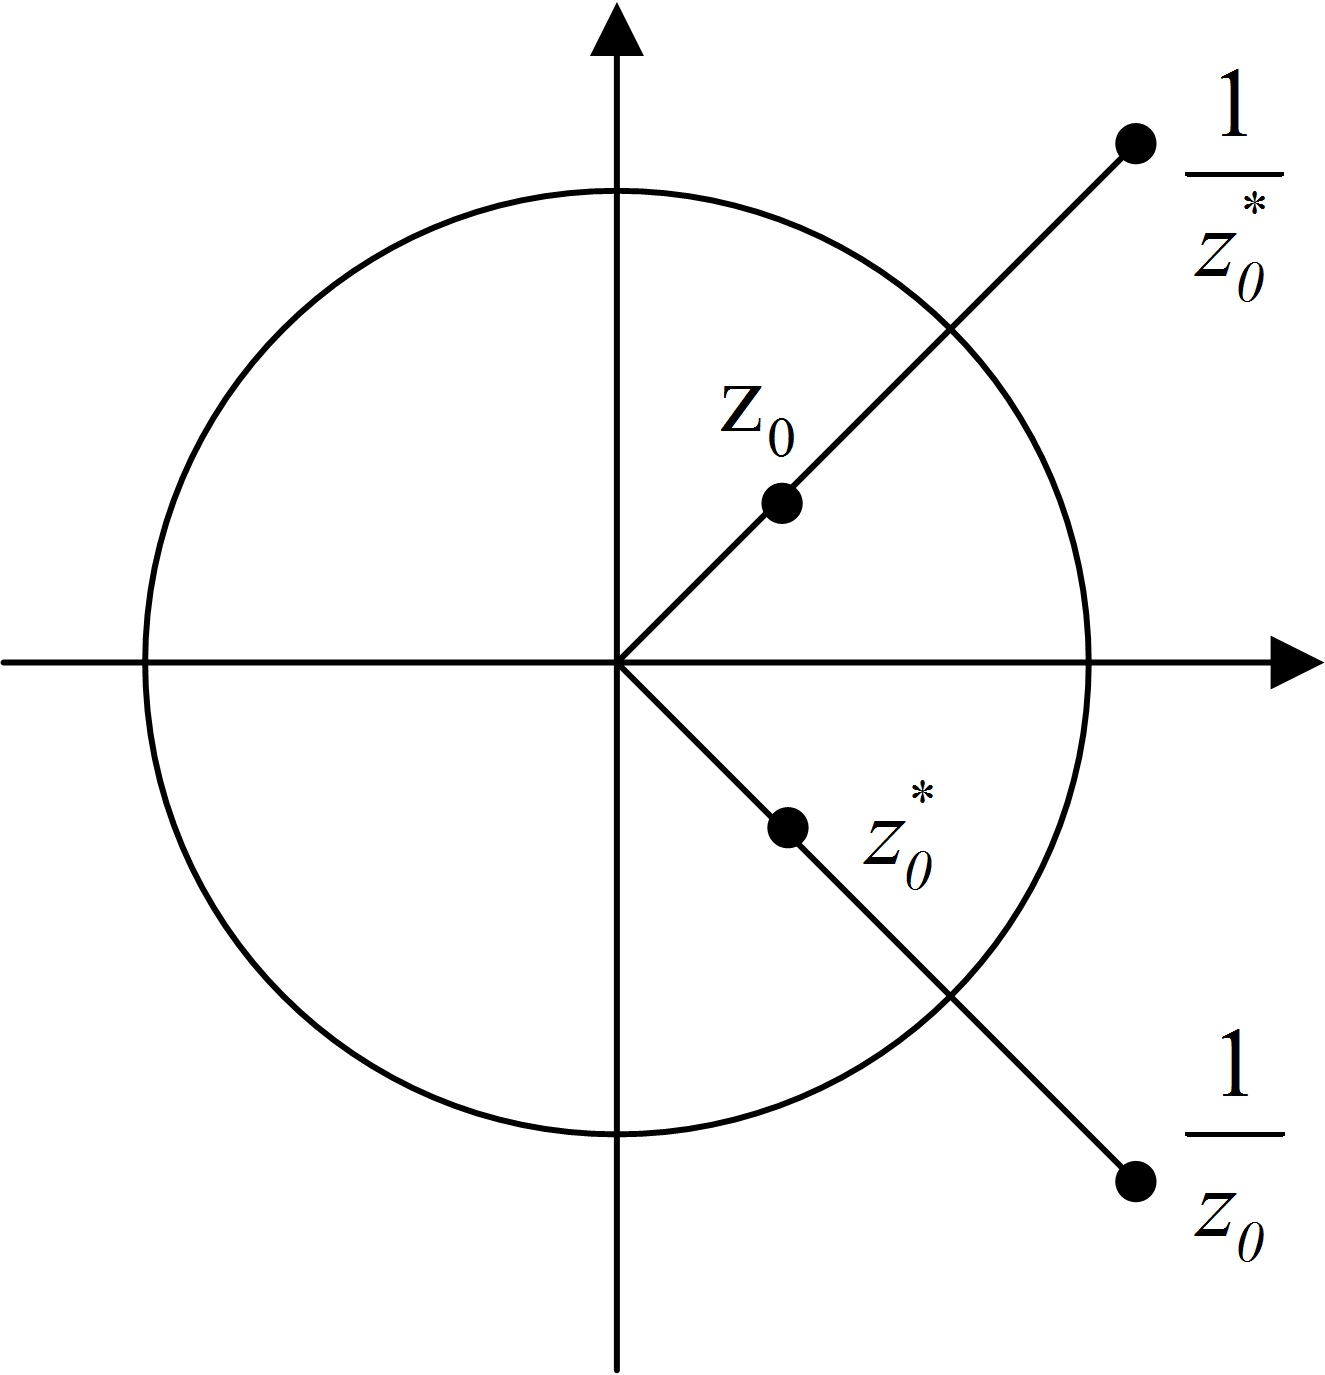
\includegraphics[width=0.35\textwidth]{xxxwldsyt.jpg}
%\caption{线性相位结构的零点分布图}
%\label{}
\end{figure}
\end{frame}
%%%%%%%%%%%%%%%%%%%%%%%%%%%%%%%%%%%%%%%%%%%%%%%%%%%%%%%%%%%%%%%%%%%%%%%%%%%%%%%%%%%%%%%%%%%%%%%


%%%%%%%%%%%%%%%%%%%%%%%%%%%%%%%%%%%%%%%%%%%%%%%%%%%%%%%%%%%%%%%%%%%%%%%%%%%%%%%%%%%%%%%%%%%%%%
\begin{frame}\frametitle{}%[allowframebreaks][shrink]
\begin{example}
     某一FIR-DF,$H(z)=\frac{1}{10}(1+2z^{-1}+4z^{-2}+2z^{-3}+z^{-4})$
     \par(1) 判断其是否具有线性相位;
     \par(2) 求出$H_g(\omega)$,$\theta(\omega)$。
     \par(3) 画出其直接型网络结构以及线性相位网络结构。
\end{example}
\end{frame}
%%%%%%%%%%%%%%%%%%%%%%%%%%%%%%%%%%%%%%%%%%%%%%%%%%%%%%%%%%%%%%%%%%%%%%%%%%%%%%%%%%%%%%%%%%%%%%%


%%%%%%%%%%%%%%%%%%%%%%%%%%%%%%%%%%%%%%%%%%%%%%%%%%%%%%%%%%%%%%%%%%%%%%%%%%%%%%%%%%%%%%%%%%%%%%
\begin{frame}[allowframebreaks]\frametitle{}%[allowframebreaks][shrink]
\par 解:\par
     \par (1)依题意,有$h(n)= \frac{1}{10}\{1,2,4,2,1\}$,
     \par 即$N=5,\quad h(n)=h(N-1-n)$,为第一类线性相位结构。
     \par (2)
     \begin{equation*}
            \begin{split}
            H(e^{j\omega})
              &= H(z)|_{z=e^{j\omega}}\\
              &= \frac{1}{10}
                 \Big(1+2e^{-j\omega}+4e^{-j2\omega}+2e^{-j3\omega}+e^{-j4\omega}\Big)\\
              &= \frac{1}{10}e^{-j2\omega}
                 \Big(e^{j2\omega}+2e^{j\omega}+4+2e^{-j\omega}+e^{-j2\omega}\Big)\\
              &= \frac{1}{10}e^{-j2\omega}\Big[4+4cos(\omega)+2cos(2\omega)\Big]\\
            \end{split}
     \end{equation*}
     $$
            \left\{ \begin{aligned}
              H_g(\omega)
                    &=\frac{1}{10}\big[4+4cos(\omega)+2cos(2\omega)\big]\qquad\qquad\qquad\quad\\
              \varphi(\omega)
                    &=-2\omega\quad(\tau = \frac{N-1}{2})\\
            \end{aligned} \right.
     $$
     \begin{figure}[h]
          \centering
          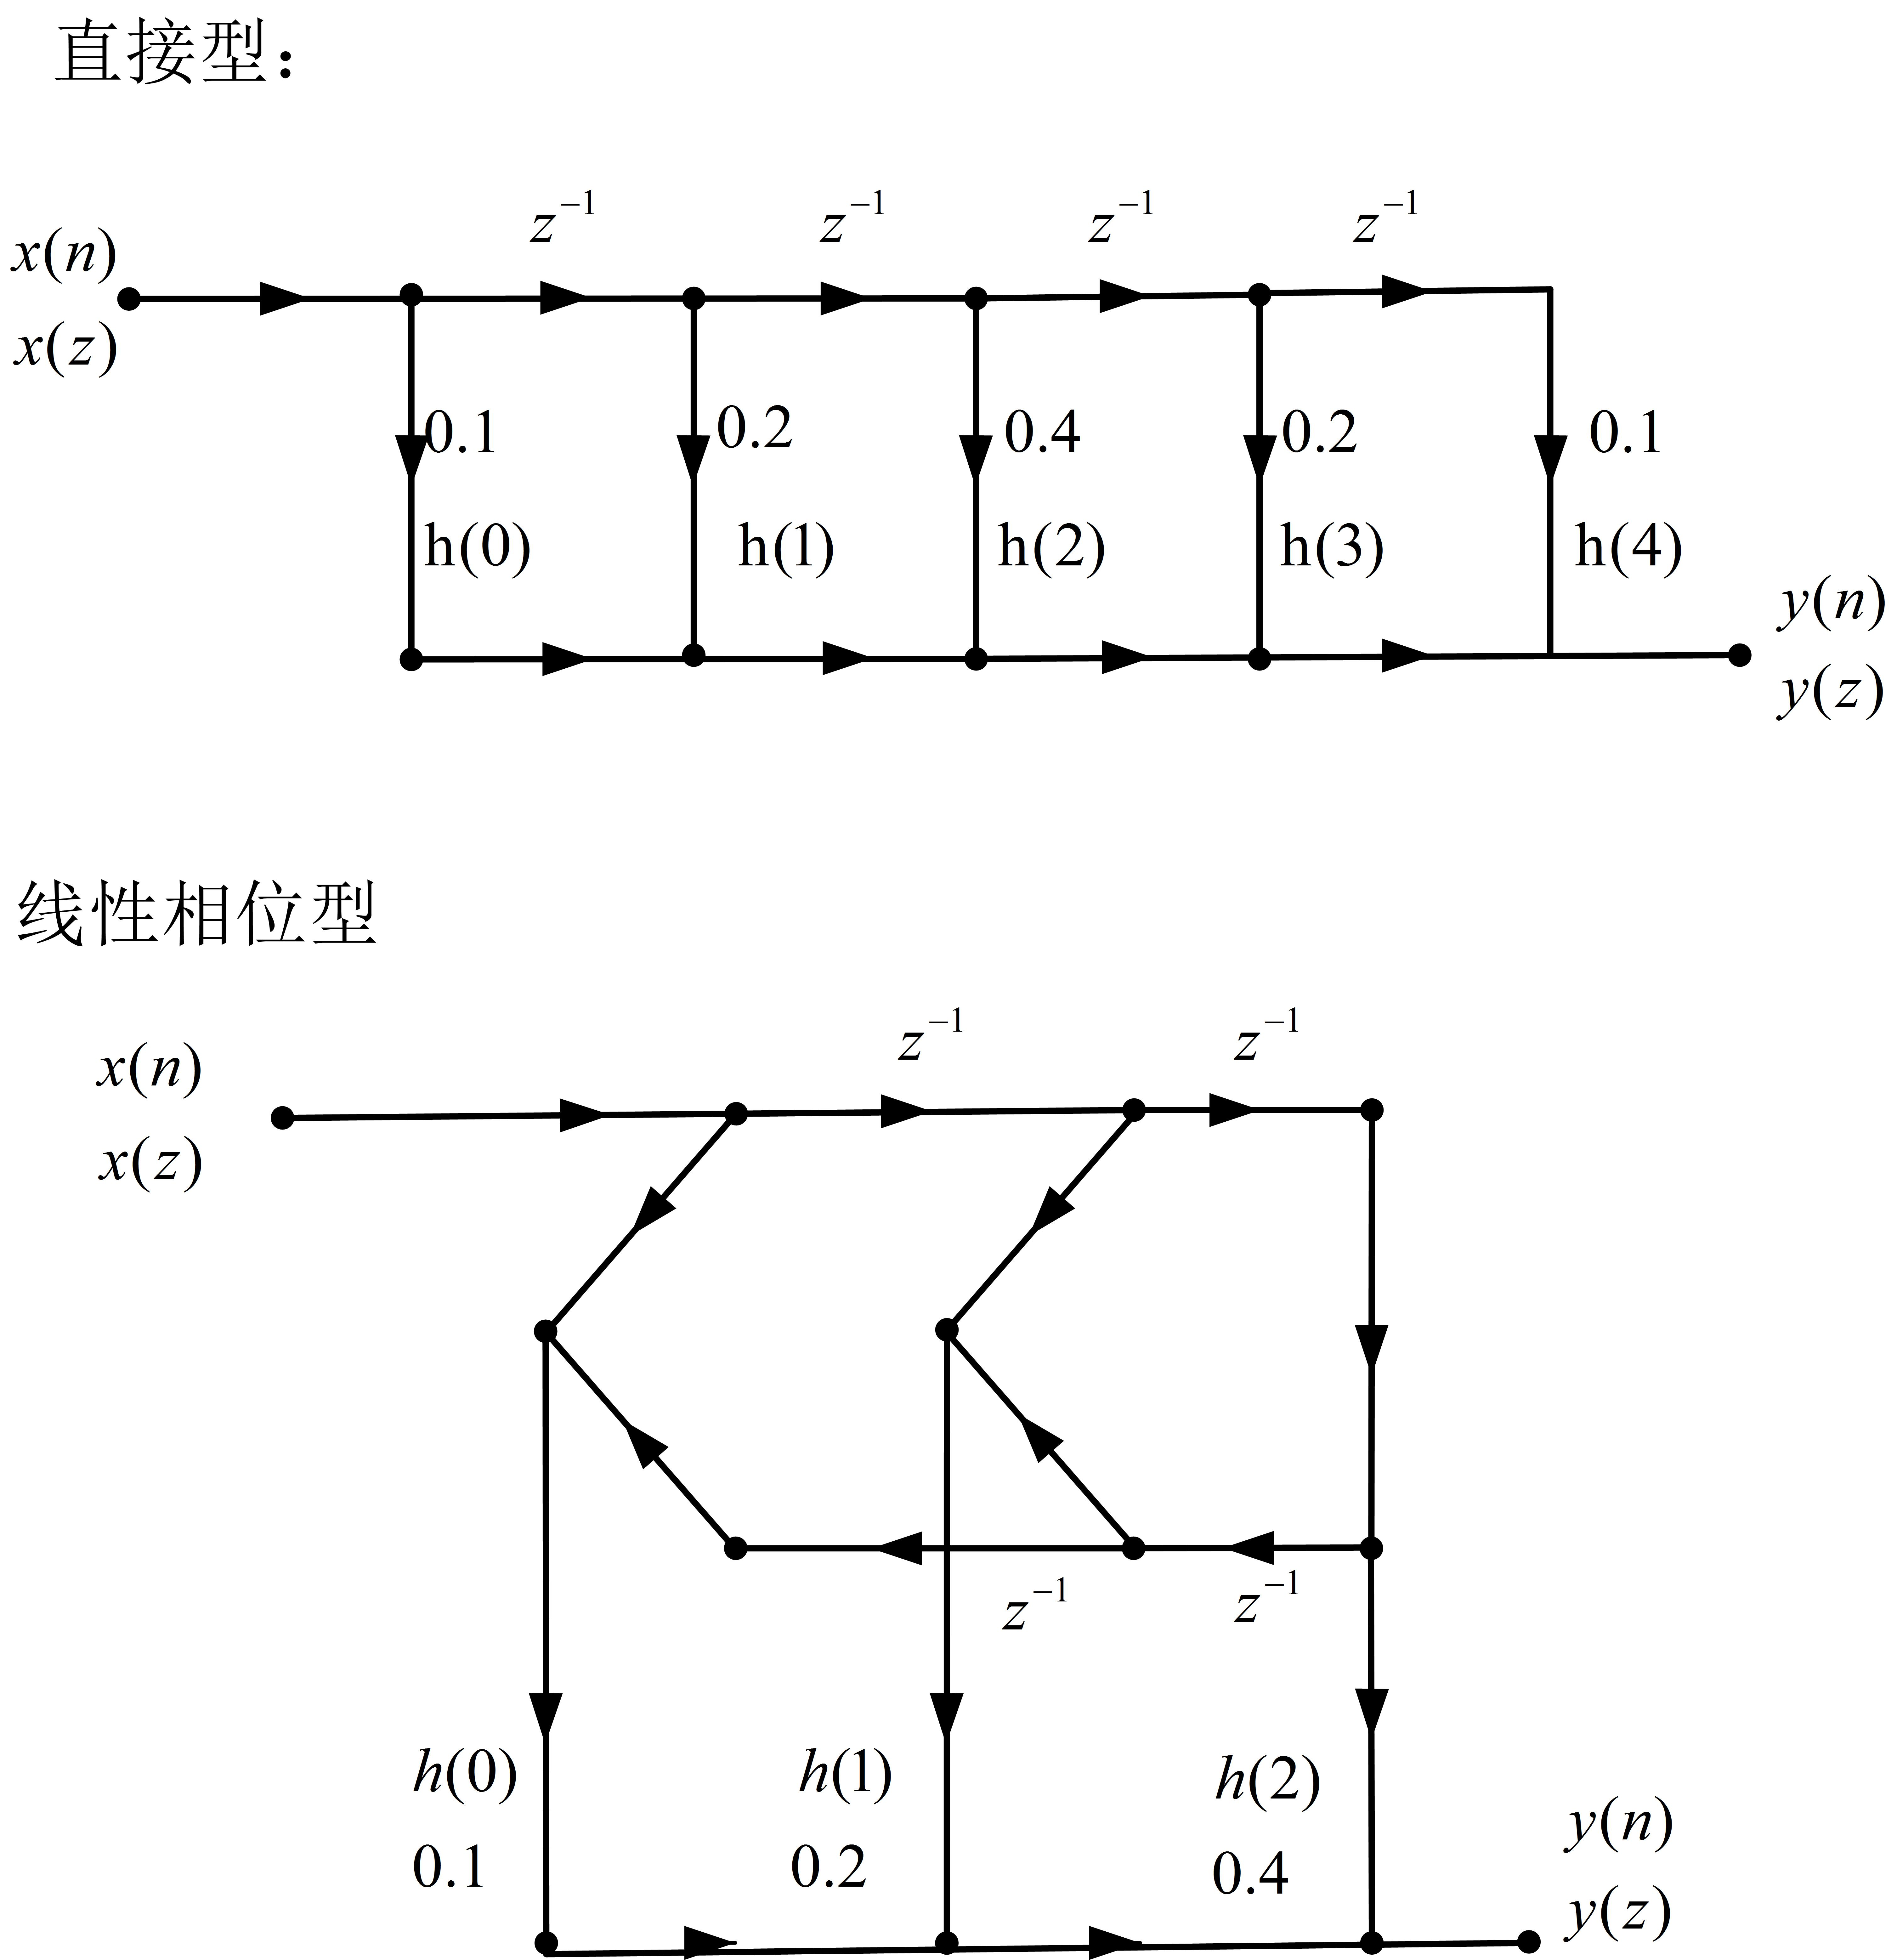
\includegraphics[width=0.7\textwidth]{example1.jpg}
          %\caption{该滤波器的网络结构}
          %\vspace{-0.8cm}
      \end{figure}


\end{frame}
%%%%%%%%%%%%%%%%%%%%%%%%%%%%%%%%%%%%%%%%%%%%%%%%%%%%%%%%%%%%%%%%%%%%%%%%%%%%%%%%%%%%%%%%%%%%%%%


%%%%%%%%%%%%%%%%%%%%%%%%%%%%%%%%%%%%%%%%%%%%%%%%%%%%%%%%%%%%%%%%%%%%%%%%%%%%%%%%%%%%%%%%%%%%%%%
%\begin{frame}\frametitle{title}%[allowframebreaks][shrink]
%
%\end{frame}
%%%%%%%%%%%%%%%%%%%%%%%%%%%%%%%%%%%%%%%%%%%%%%%%%%%%%%%%%%%%%%%%%%%%%%%%%%%%%%%%%%%%%%%%%%%%%%%
\section{用窗函数法设计FIR-DF}
\begin{frame}\frametitle{7.3  用窗函数法设计FIR-DF}%[allowframebreaks][shrink]

\end{frame}

\subsection{概述}

%%%%%%%%%%%%%%%%%%%%%%%%%%%%%%%%%%%%%%%%%%%%%%%%%%%%%%%%%%%%%%%%%%%%%%%%%%%%%%%%%%%%%%%%%%%%%%
\begin{frame}\frametitle{7.3.1 概述}%[allowframebreaks][shrink]
 在IIR-DF设计方法中,我们
   \begin{itemize}
       \item 用实际滤波器$\quad\underrightarrow{\quad\mbox{逼近}
                    \quad}\quad$理想滤波器。
       \item 当所涉及的实际滤波器满足技术要求时,停止逼近。
   \end{itemize}

   在FIR-DF设计中,我们希望设计长度为N的$h(n)$,希望:
      \begin{enumerate}
        \item 具有线性相位
        \item 能逼近理想DF
      \end{enumerate}
   不同的是,我们将直接对理想滤波器进行处理得到。
\end{frame}
%%%%%%%%%%%%%%%%%%%%%%%%%%%%%%%%%%%%%%%%%%%%%%%%%%%%%%%%%%%%%%%%%%%%%%%%%%%%%%%%%%%%%%%%%%%%%%%
\subsection{窗函数法设计原理}

%%%%%%%%%%%%%%%%%%%%%%%%%%%%%%%%%%%%%%%%%%%%%%%%%%%%%%%%%%%%%%%%%%%%%%%%%%%%%%%%%%%%%%%%%%%%%%
\begin{frame}[shrink]\frametitle{7.3.2 窗函数法设计原理}%[allowframebreaks][shrink]

  \textbf{一、 理想滤波器}
  \par
       \begin{figure}[h]
           \centering
           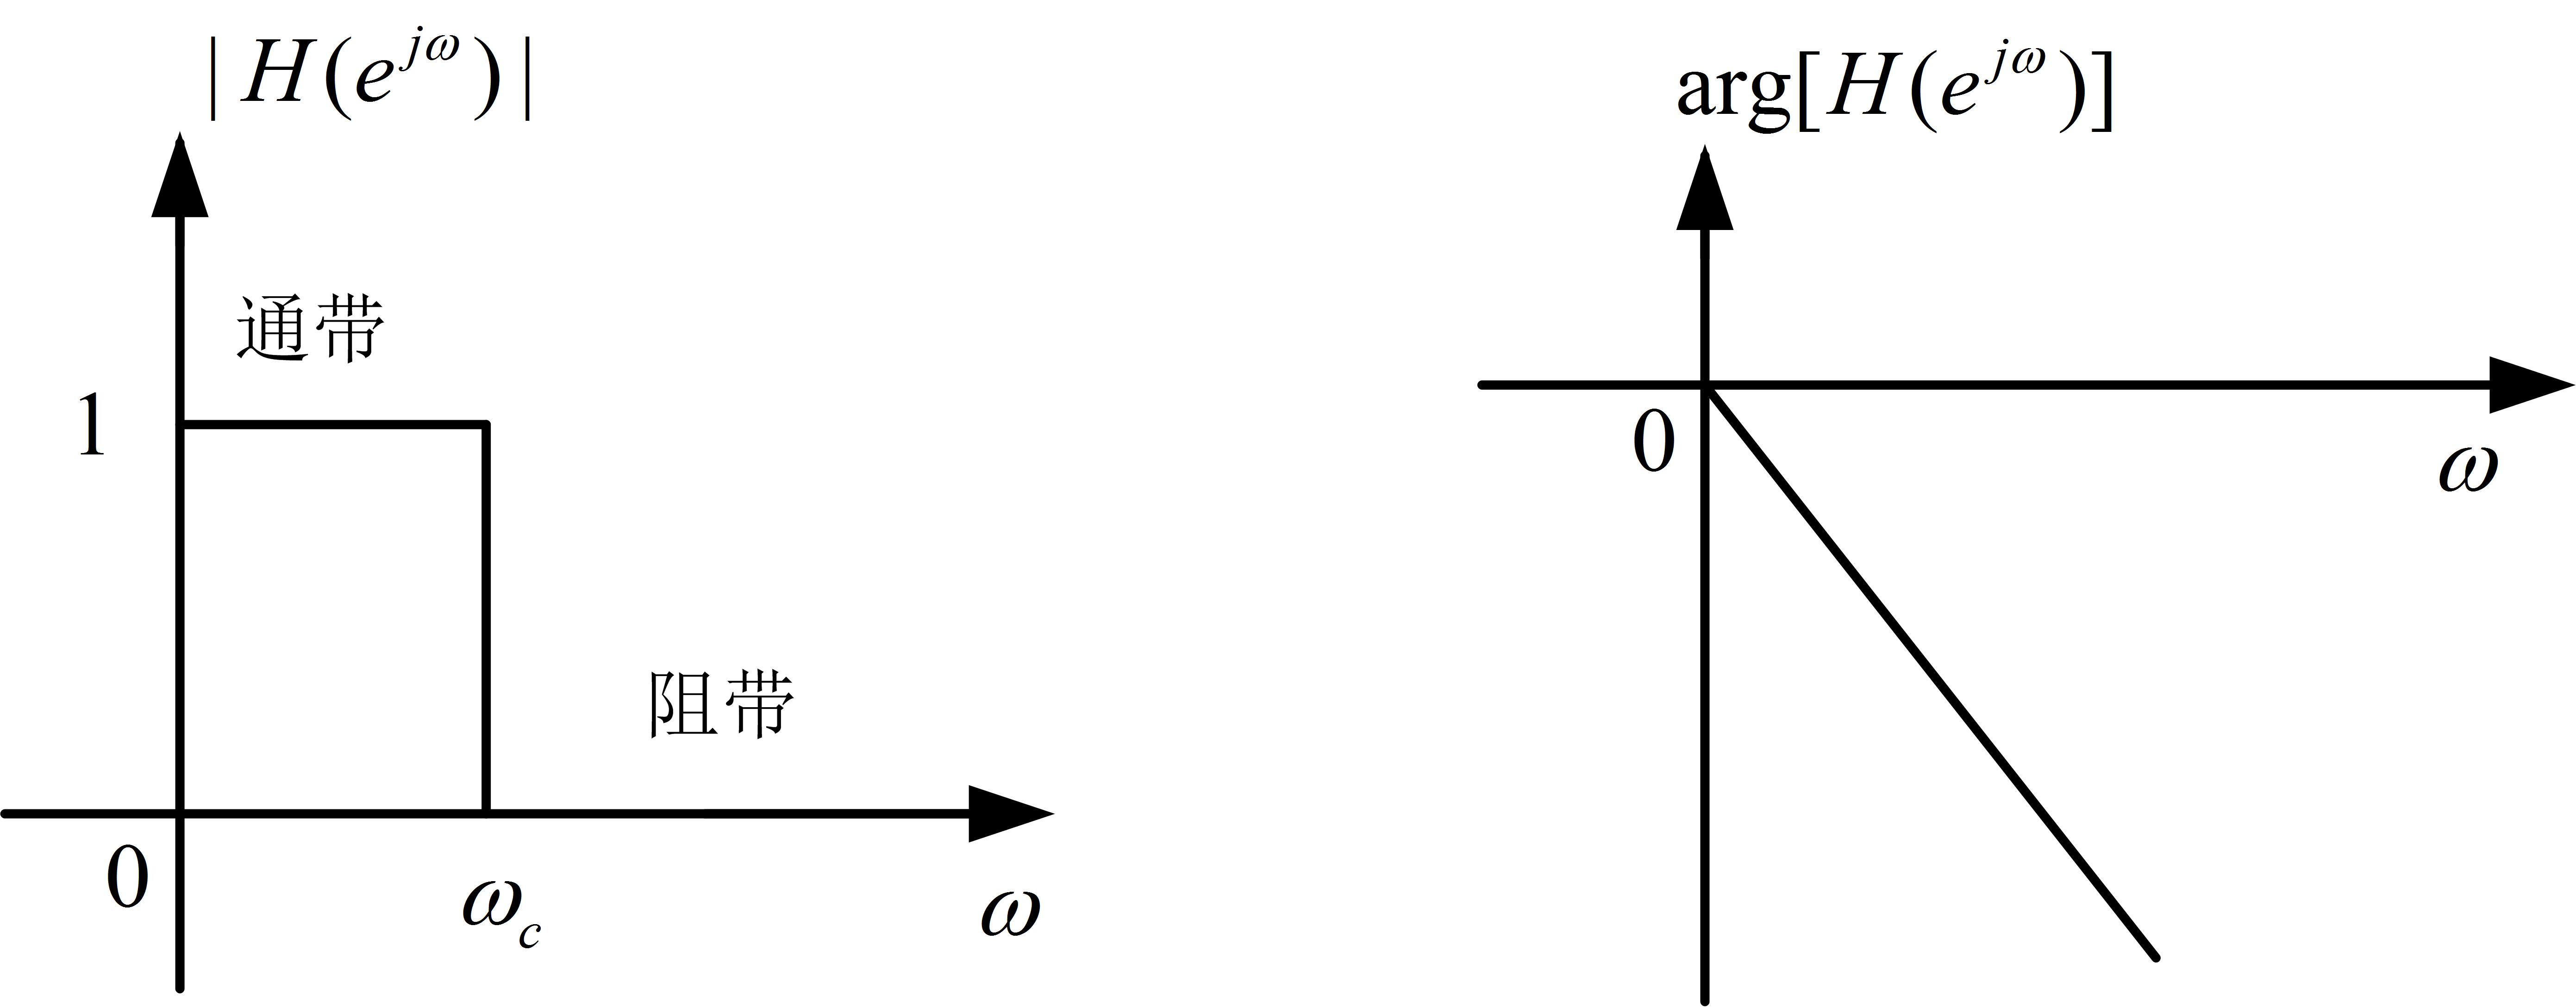
\includegraphics[width=0.7\textwidth]{fig2lxlbqtx.jpg}
           \caption{理想滤波器的幅频特性与相频特性}
          %\label{}
       \end{figure}
      则线性相位理想低通滤波器为:
      $$
        H_d(e^{j\omega}) =
        \left\{\begin{array}
             {r@{,\quad}l}
             e^{-j\omega\alpha} & \quad\quad|\omega|\leqslant \omega_c\quad\quad\\
             0 \quad\quad       & \omega_c<|\omega|\leqslant \pi
        \end{array} \right.
      $$
\end{frame}
%%%%%%%%%%%%%%%%%%%%%%%%%%%%%%%%%%%%%%%%%%%%%%%%%%%%%%%%%%%%%%%%%%%%%%%%%%%%%%%%%%%%%%%%%%%%%%%


%%%%%%%%%%%%%%%%%%%%%%%%%%%%%%%%%%%%%%%%%%%%%%%%%%%%%%%%%%%%%%%%%%%%%%%%%%%%%%%%%%%%%%%%%%%%%%
\begin{frame}[shrink]\frametitle{}%[allowframebreaks][shrink]
     \textbf{二、 求$h_d(n)$}\par
     线性相位理想低通滤波器为:
      $$
        H_d(e^{j\omega}) =
        \left\{\begin{array}
             {r@{,\quad}l}
             e^{-j\omega\alpha} & \quad\quad|\omega|\leqslant \omega_c\quad\quad\\
             0 \quad\quad       & \omega_c<|\omega|\leqslant \pi
        \end{array} \right.
      $$

      \begin{center}
      令:$\quad\quad h_d(n)\longleftrightarrow H_d(e^{j\omega})\quad\quad\quad\quad\quad\quad$
      \end{center}


      $$
        \left\{ \begin{aligned}
          H_{dg}(\omega) &=1\quad\quad\quad |\omega|\leqslant \omega_c\\
          \theta(\omega)\quad &=-\alpha\omega\\
        \end{aligned} \right.
      $$

      $$
        \left\{ \begin{aligned}
          H_d(e^{j\omega})
             &=\sum_{n=-\infty}^{\infty}h_d(n)e^{-j\omega n}\\
          h_d(n)
             &=\frac{1}{2\pi}\int_{-\pi}^{\pi}H_d(e^{j\omega})e^{j\omega n}d\omega\\
        \end{aligned} \right.
      $$
      显然,可通过直接对$H_d(e^{j\omega})$做反变换求$h_d(n)$。

\end{frame}
%%%%%%%%%%%%%%%%%%%%%%%%%%%%%%%%%%%%%%%%%%%%%%%%%%%%%%%%%%%%%%%%%%%%%%%%%%%%%%%%%%%%%%%%%%%%%%%


%%%%%%%%%%%%%%%%%%%%%%%%%%%%%%%%%%%%%%%%%%%%%%%%%%%%%%%%%%%%%%%%%%%%%%%%%%%%%%%%%%%%%%%%%%%%%%
\begin{frame}[shrink]\frametitle{}%[allowframebreaks][shrink]
$$h_d(n)=\frac{1}{2\pi}\int_{-\pi}^{\pi}H_d(e^{j\omega})e^{j\omega n}d\omega$$

      则有:
      \begin{equation*}
        \begin{split}
        h_d(n)
          &=\frac{1}{2\pi}\int_{-\omega_c}^{\omega_c}
             e^{-j\omega\alpha}e^{j\omega n}d\omega\\
          &=\frac{sin\left[\omega_c(n-\alpha)\right]}{\pi(n-\alpha)}
           =\frac{\omega_c}{\pi}\frac{sin\left[\omega_c(n-\alpha)\right]}
            {\omega_c(n-\alpha)}\\
          &=\frac{\omega_c}{\pi}Sa\left[\omega_c(n-\alpha)\right]
        \end{split}
      \end{equation*}
\end{frame}
%%%%%%%%%%%%%%%%%%%%%%%%%%%%%%%%%%%%%%%%%%%%%%%%%%%%%%%%%%%%%%%%%%%%%%%%%%%%%%%%%%%%%%%%%%%%%%%


%%%%%%%%%%%%%%%%%%%%%%%%%%%%%%%%%%%%%%%%%%%%%%%%%%%%%%%%%%%%%%%%%%%%%%%%%%%%%%%%%%%%%%%%%%%%%%
\begin{frame}[shrink]\frametitle{}%[allowframebreaks][shrink]
$$h_d(n)=\frac{\omega_c}{\pi}Sa\left[\omega_c(n-\alpha)\right]$$
\begin{figure}[h]
    \centering
    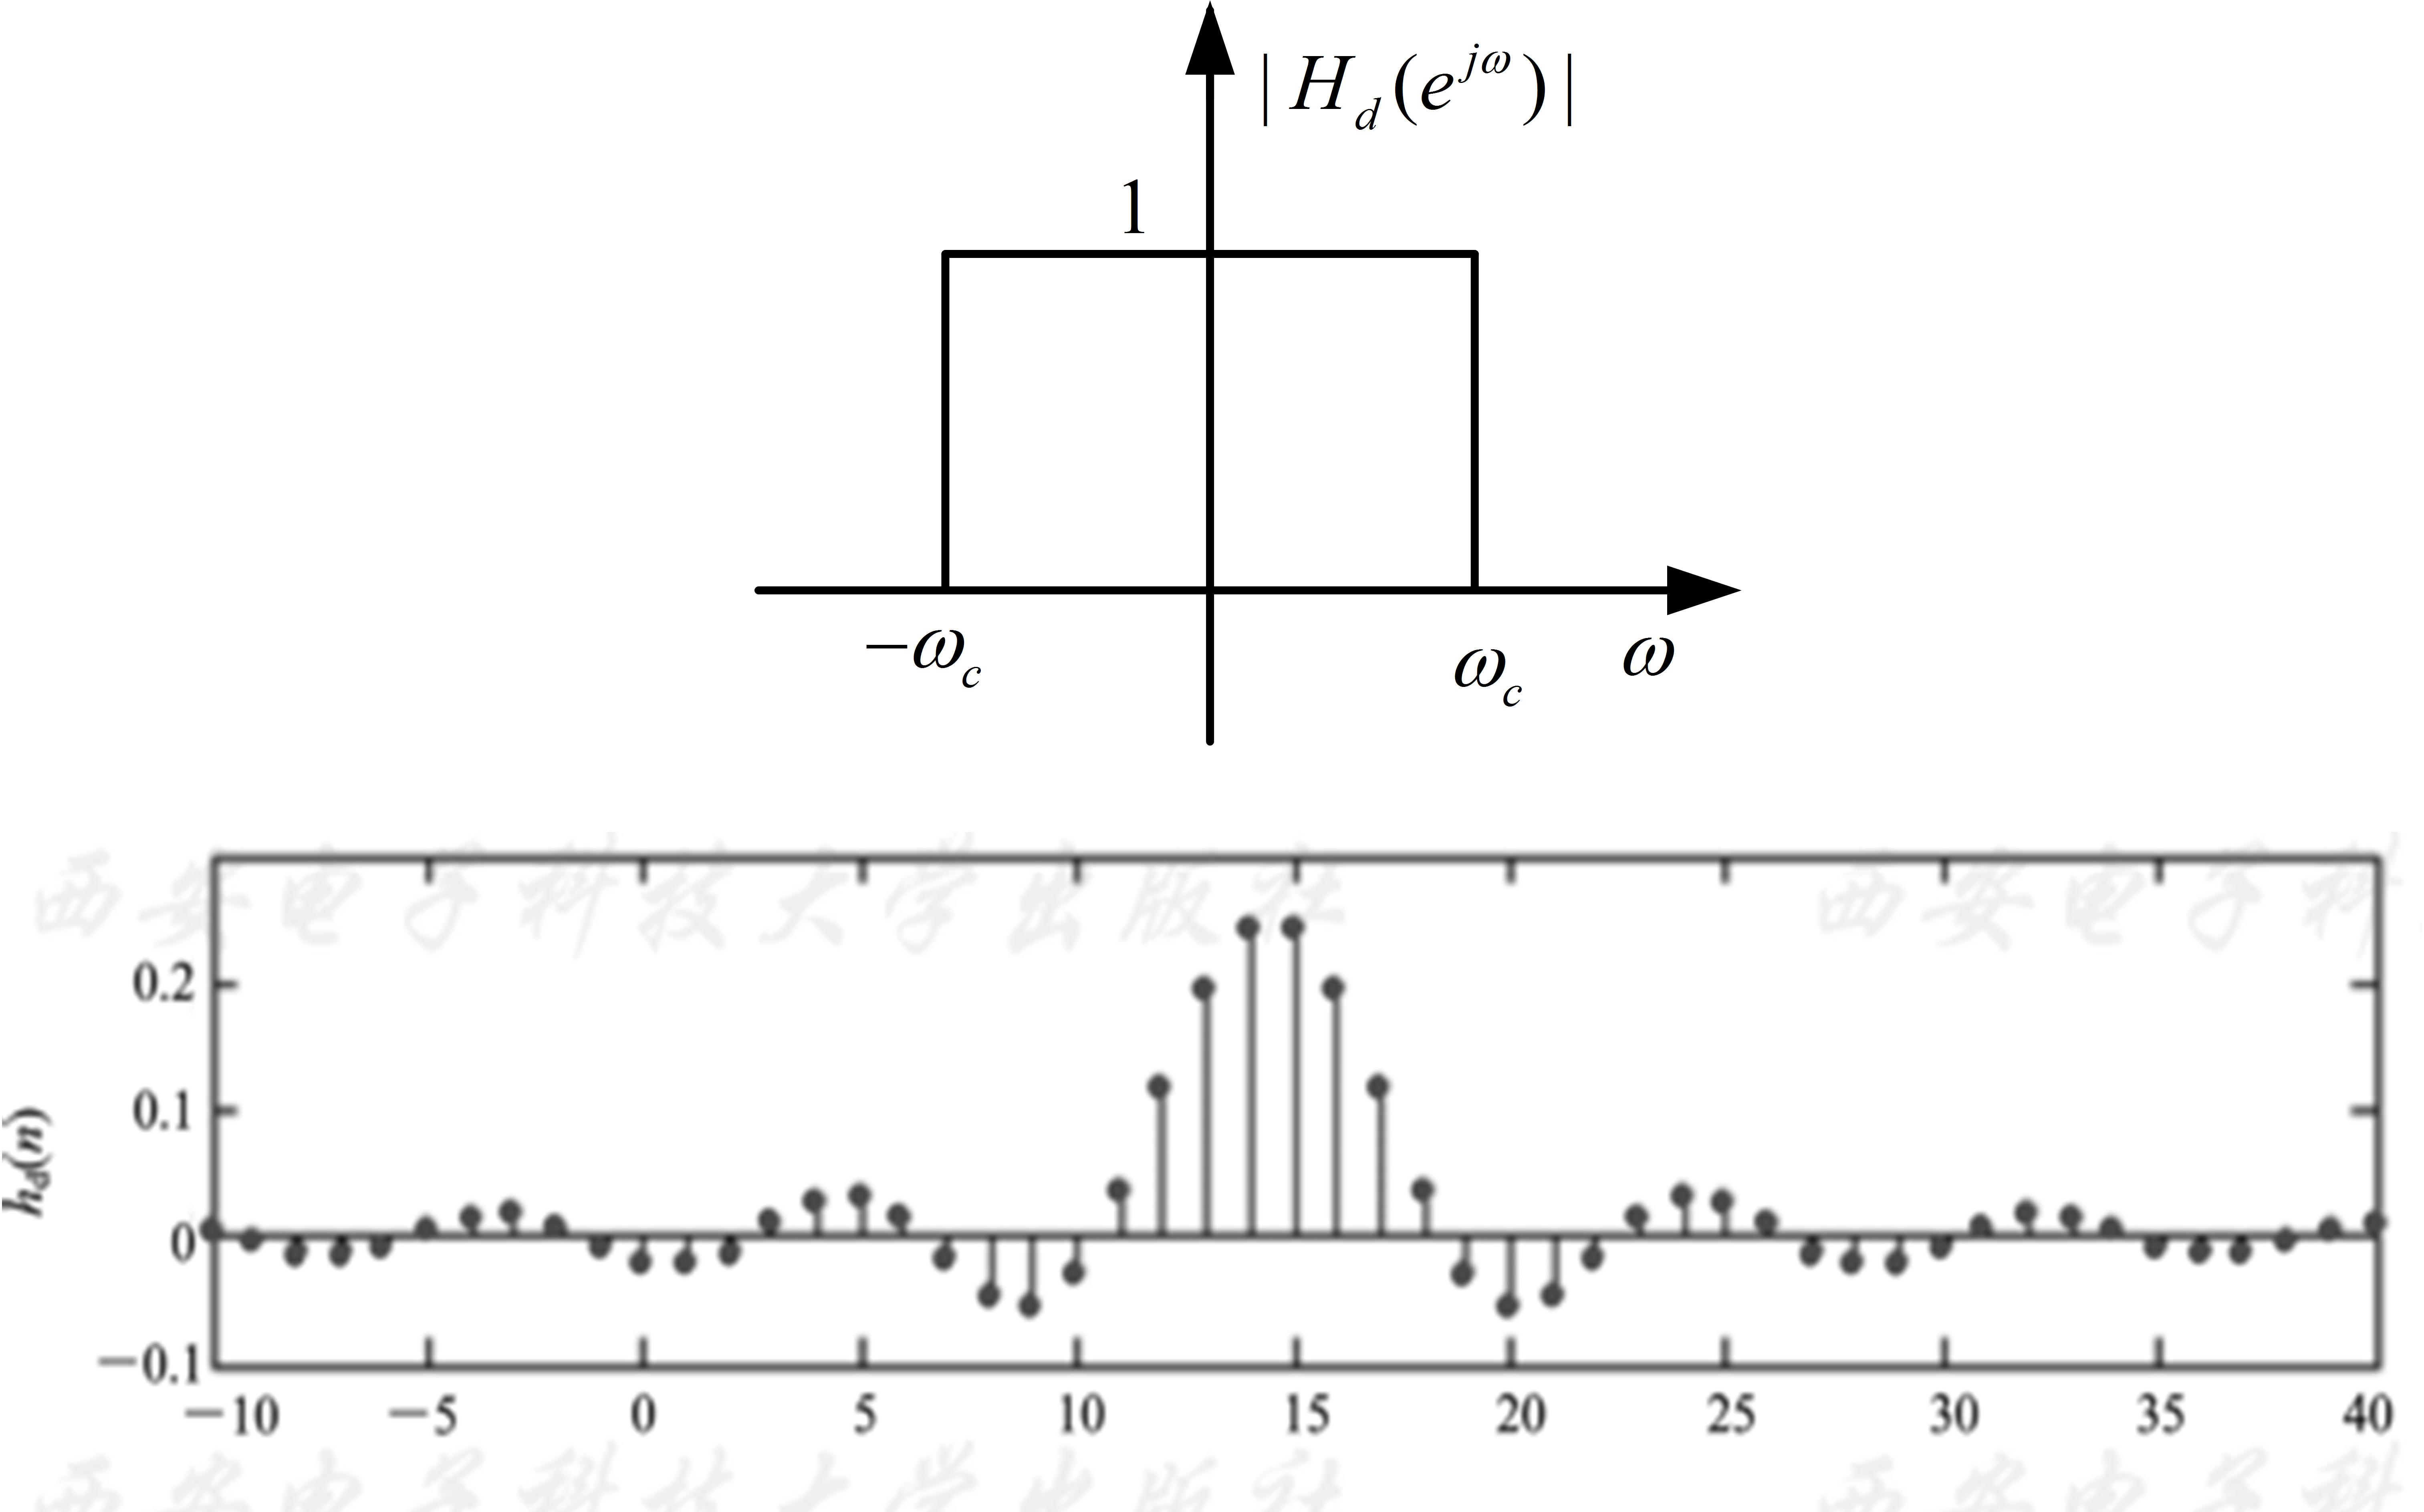
\includegraphics[width=0.7\textwidth]{fig1_lixianglvboqi.jpg}
    %\caption{线性相位理想滤波器示意图}
    %\label{}
\end{figure}
显然$h_d(n)$无限长,非因果。
\end{frame}
%%%%%%%%%%%%%%%%%%%%%%%%%%%%%%%%%%%%%%%%%%%%%%%%%%%%%%%%%%%%%%%%%%%%%%%%%%%%%%%%%%%%%%%%%%%%%%%


%%%%%%%%%%%%%%%%%%%%%%%%%%%%%%%%%%%%%%%%%%%%%%%%%%%%%%%%%%%%%%%%%%%%%%%%%%%%%%%%%%%%%%%%%%%%%%
\begin{frame}\frametitle{}%[allowframebreaks][shrink]

三、用窗函数法设计FIR-DF的方法:
      \begin{enumerate}
        \item 对$h_d(n)$截取一段,得到$h(n)$
        \item 使得$h(n)$具有线性相位。(条件:$h(n) = h(N-1-n)$
        \item 必须令$\alpha = \frac{N-1}{2}$
      \end{enumerate}
\end{frame}
%%%%%%%%%%%%%%%%%%%%%%%%%%%%%%%%%%%%%%%%%%%%%%%%%%%%%%%%%%%%%%%%%%%%%%%%%%%%%%%%%%%%%%%%%%%%%%%


%%%%%%%%%%%%%%%%%%%%%%%%%%%%%%%%%%%%%%%%%%%%%%%%%%%%%%%%%%%%%%%%%%%%%%%%%%%%%%%%%%%%%%%%%%%%%%
\begin{frame}\frametitle{}%[allowframebreaks][shrink]



  \textbf{四、 问题:}

      $h(n)$是对$h_d(n)$截取得到得到,必定存在误差。

      表现为:吉布斯效应。\emph{这种吉布斯效应是由于将$h_d(n)$ 截断引起的,也叫截断效应。}



\end{frame}
%%%%%%%%%%%%%%%%%%%%%%%%%%%%%%%%%%%%%%%%%%%%%%%%%%%%%%%%%%%%%%%%%%%%%%%%%%%%%%%%%%%%%%%%%%%%%%%

\subsection{$h(n)$的幅度特性与截断效应}
%%%%%%%%%%%%%%%%%%%%%%%%%%%%%%%%%%%%%%%%%%%%%%%%%%%%%%%%%%%%%%%%%%%%%%%%%%%%%%%%%%%%%%%%%%%%%%
\begin{frame}\frametitle{7.3.3 $h(n)$的幅度特性与截断效应}%[allowframebreaks][shrink]


    显然有
    $$h(n) = h_d(n)R_N(n) \quad\quad\quad\quad\quad   h(n)\longleftrightarrow H(e^{j\omega})$$
\begin{enumerate}
  \item [1] 幅度特性
\end{enumerate}
    $$\mbox{令:}\quad\quad H(e^{j\omega})   = H_g(\omega)e^{j\varphi_1(\omega)}\quad\quad\quad\quad
    \quad\quad$$
    \begin{equation*}
    \begin{split}
    \mbox{设:}\quad\quad
        h_d(n)  &\longleftrightarrow H_d(e^{j\omega}) = H_{dg}(\omega)e^{j\varphi_2(\omega)}\\
        R_N(n)  &\longleftrightarrow R_N(e^{j\omega}) =R_{Ng}(\omega)e^{j\varphi_3(\omega)}
    \end{split}
    \end{equation*}
\end{frame}
%%%%%%%%%%%%%%%%%%%%%%%%%%%%%%%%%%%%%%%%%%%%%%%%%%%%%%%%%%%%%%%%%%%%%%%%%%%%%%%%%%%%%%%%%%%%%%%


%%%%%%%%%%%%%%%%%%%%%%%%%%%%%%%%%%%%%%%%%%%%%%%%%%%%%%%%%%%%%%%%%%%%%%%%%%%%%%%%%%%%%%%%%%%%%%
\begin{frame}\frametitle{}%[allowframebreaks][shrink]

    下面推导$h(n)$对应的$H_g(\omega)$的特性。
    $$\mbox{因:}\quad\quad\quad\quad h(n) = h_d(n)R_N(n) \quad\quad\quad\quad\quad\quad\quad\quad\quad\quad$$
    \begin{equation*}
        \begin{split}
        H(e^{j\omega})
          &=\frac{1}{2\pi}H_d(e^{j\omega})\ast R_N(e^{j\omega})\\
          &=\frac{1}{2\pi}\int_{-\pi}^{\pi}H_d(e^{j\theta})R_N(e^{j(\omega -\theta)})d\theta
        \end{split}
      \end{equation*}
    \begin{itemize}
      \item[(a)] 窗函数傅里叶变换$R_N(e^{j\omega})$的幅度特性与相位特性
    \end{itemize}
        $$R_N(e^{j\omega}) = \sum_{n=0}^{N-1}R_N(n)e^{-j\omega n}= e^{-j\frac{N-1}{2}\omega}
        \frac{sin(\frac{N}{2}\omega)}{sin(\frac{\omega}{2})}$$
        $$\therefore\quad\quad
        R_{Ng}(\omega) = \frac{sin(\frac{N}{2}\omega)}{sin(\frac{\omega}{2})}\quad\quad
        \varphi_3(\omega) = -\frac{N-1}{2}\omega = -\alpha\omega$$
\end{frame}
%%%%%%%%%%%%%%%%%%%%%%%%%%%%%%%%%%%%%%%%%%%%%%%%%%%%%%%%%%%%%%%%%%%%%%%%%%%%%%%%%%%%%%%%%%%%%%%


%%%%%%%%%%%%%%%%%%%%%%%%%%%%%%%%%%%%%%%%%%%%%%%%%%%%%%%%%%%%%%%%%%%%%%%%%%%%%%%%%%%%%%%%%%%%%%
\begin{frame}\frametitle{}%[allowframebreaks][shrink]

      \begin{itemize}
      \item[(b)] 理想滤波器$H_d(e^{j\omega})$的幅度特性与相位特性
      \end{itemize}
          设:
          $$
            H_d(e^{j\omega}) =
            \left\{\begin{array}
                 {r@{,\quad}l}
                 e^{-j\omega\alpha} & \quad\quad\quad|\omega|\leqslant \omega_c\\
                 0                  & \quad\omega_c<|\omega|\leqslant \pi
            \end{array} \right.
          $$
          显然有:
          $$
            H_{dg}(\omega) =
            \left\{\begin{array}
                 {r@{,\quad}l}
                 1 & \quad\quad\quad|\omega|\leqslant \omega_c\\
                 0 & \quad\omega_c<|\omega|\leqslant \pi
            \end{array} \right.
          $$
          $$\therefore\quad\quad \varphi_2(\omega) = -\alpha\omega
          \quad\quad\quad\quad\quad\quad\quad\quad\quad\quad\quad\quad$$
\end{frame}
%%%%%%%%%%%%%%%%%%%%%%%%%%%%%%%%%%%%%%%%%%%%%%%%%%%%%%%%%%%%%%%%%%%%%%%%%%%%%%%%%%%%%%%%%%%%%%%


%%%%%%%%%%%%%%%%%%%%%%%%%%%%%%%%%%%%%%%%%%%%%%%%%%%%%%%%%%%%%%%%%%%%%%%%%%%%%%%%%%%%%%%%%%%%%%
\begin{frame}\frametitle{}%[allowframebreaks][shrink]

          将$(a),(b)$的结果代入公式(*)得:
          \begin{equation*}
            \begin{split}
            H(e^{j\omega})
              &= \frac{1}{2\pi}\int_{-\pi}^{\pi}
                 \left[H_{dg}(\theta)e^{j\varphi_2(\theta)})\right]
                 \left[R_{Ng}(\omega-\theta)e^{j\varphi_3(\omega-\theta)}\right]
                 d\theta\\
              &= \frac{1}{2\pi}\int_{-\pi}^{\pi}
                 \left[H_{dg}(\theta)e^{-j\alpha\theta}\right]
                 \left[R_{Ng}(\omega-\theta)e^{-j\alpha(\omega-\theta)}\right]
                 d\theta\\
              &= e^{-j\alpha\omega}\frac{1}{2\pi}\int_{-\pi}^{\pi}
                 H_{dg}(\theta)R_{Ng}(\omega-\theta)d\theta\\
              &= e^{-j\alpha\omega}\Big[\frac{1}{2\pi} H_{dg}(\omega)\ast R_{Ng}(\omega)\Big]\\
            \end{split}
          \end{equation*}
          $$
            \left\{ \begin{aligned}
              H_g(\omega)
                    &=\frac{1}{2\pi}\int_{-\pi}^{\pi}
                 H_{dg}(\theta)R_{Ng}(\omega-\theta)d\theta \\%= H_{dg}(\omega)\ast R_{Ng}(\omega)\\
              \varphi_1(\omega)
                    &=-\alpha\omega\\
            \end{aligned} \right.
          $$

          即:$h(n)$的幅度特性$H_g(\omega)$是窗函数幅度特性$R_{Ng}(\omega)$
          与理想滤波器幅度特性$H_{dg}(\omega)$的卷积

\end{frame}
%%%%%%%%%%%%%%%%%%%%%%%%%%%%%%%%%%%%%%%%%%%%%%%%%%%%%%%%%%%%%%%%%%%%%%%%%%%%%%%%%%%%%%%%%%%%%%%


%%%%%%%%%%%%%%%%%%%%%%%%%%%%%%%%%%%%%%%%%%%%%%%%%%%%%%%%%%%%%%%%%%%%%%%%%%%%%%%%%%%%%%%%%%%%%%
\begin{frame}[allowframebreaks]\frametitle{}%[allowframebreaks][shrink]
\begin{enumerate}
\item [2] 截断效应的产生:
\end{enumerate}

      $$\mbox{即:}\quad H_{dg}(\omega)\ast R_{Ng}(\omega)\quad\mbox{形成}\quad H_g(\omega)\quad\mbox{的过程。}$$
      $$p223:\quad\quad
      (a)\ast (b)\longrightarrow (f)
      \quad\quad\mbox{的过程}$$
      \begin{enumerate}
        \item[(1)] $\omega=0$
        \begin{equation*}
            \begin{split}
            H_g(0)
              &= \frac{1}{2\pi}\int_{-\pi}^{\pi}
                 H_{dg}(\theta)R_{Ng}(\omega-\theta)d\theta |_{\omega=0}
              = \frac{1}{2\pi}\int_{-\omega_c}^{\omega_c}%H_{dg}(\theta)
                 R_{Ng}(\theta)d\theta\\
            \end{split}
        \end{equation*}
          即为$R_{Ng}(\omega)$在$(-\omega_c,\omega_c )$之间的积分,在
          $\omega_c \gg \frac{2\pi}{N}$时,相当于$(-\pi,\pi)$ 之间的积分。

          将$H_g(0)$归一化为1,下面设$\omega_c \gg \frac{2\pi}{N}$。
        \item[(2)]$\omega = \omega_c$
            $$H_g(\omega_c) \approx \frac{1}{2}H_g(0)=0.5\quad$$
            $$\mbox{即为$R_{Ng}(\omega)$在$(-\omega_c,\omega_c)$之间的积分的一半}$$
        \item[(3)] $\omega = \omega_c-\frac{2\pi}{N}$时,
            $$H_g(\omega_c-\frac{2\pi}{N}) = 1+0.0895\quad
            \mbox{(即为$H_g(\omega)$的最大值。)}$$
        \item[(4)] $\omega = \omega_c+\frac{2\pi}{N}$时,
            $$H_g(\omega_c+\frac{2\pi}{N}) = 1-0.0895\quad
            \mbox{(即为$H_g(\omega)$的最小值。}$$
      \end{enumerate}
\end{frame}
%%%%%%%%%%%%%%%%%%%%%%%%%%%%%%%%%%%%%%%%%%%%%%%%%%%%%%%%%%%%%%%%%%%%%%%%%%%%%%%%%%%%%%%%%%%%%%%


%%%%%%%%%%%%%%%%%%%%%%%%%%%%%%%%%%%%%%%%%%%%%%%%%%%%%%%%%%%%%%%%%%%%%%%%%%%%%%%%%%%%%%%%%%%%%%
\begin{frame}[allowframebreaks]\frametitle{}%[allowframebreaks][shrink]
\begin{enumerate}
\item [3] 吉布斯效应(截断效应)
\end{enumerate}
      \begin{enumerate}
      \item  吉布斯效应现象:\par
          \begin{enumerate}
            \item
                在理想特性不连续点$\omega=\omega_c$附近形成过渡带。 过渡带的宽度等于$R_{dg}(\omega)$主瓣宽度$\frac{4\pi}{N}$,
                其近似精确值为:$1.8\pi/N$
            \item
                通带内产生波纹,最大的峰值在$\omega_c-2\pi/N$处,阻带内产生了
                余振,最大的负峰在$\omega_c+2\pi/N$处。
          \end{enumerate}
      \item 吉布斯效应产生的原因
          \begin{itemize}
            \item
            $H_d(e^{j\omega})$是一个以$2\pi$为周期的函数,可以展开为傅里叶级数:
                   $$H_d(e^{j\omega}) = \sum_{n=-\infty}^{\infty}h_d(n)e^{-j\omega n}$$
                  傅里叶系数为$h_d(n)$,也就是$H_d(e^{j\omega})$对应的单位脉冲响应。这里
                  $h_d(n)$是非因果其无限长的。\par

                  窗函数法实际上是是以用N项傅里叶级数去近似无穷项傅里叶级数,这样必定会在频率不
                  连续点附近引起误差,这个误差就是所谓的吉布斯效应,也叫截断效应。
          \end{itemize}
      \end{enumerate}
\begin{enumerate}
\newpage
 \item [4] 措施
\end{enumerate}


    \begin{enumerate}
      \item 增大N

          可改善过渡带宽度,但对通带阻带的波纹改善甚微。

      \item 窗函数的选择

          选择合适的窗函数,可有效地减少通带内波动及增大阻带衰减。
    \end{enumerate}


\end{frame}
%%%%%%%%%%%%%%%%%%%%%%%%%%%%%%%%%%%%%%%%%%%%%%%%%%%%%%%%%%%%%%%%%%%%%%%%%%%%%%%%%%%%%%%%%%%%%%%


%%%%%%%%%%%%%%%%%%%%%%%%%%%%%%%%%%%%%%%%%%%%%%%%%%%%%%%%%%%%%%%%%%%%%%%%%%%%%%%%%%%%%%%%%%%%%%
\begin{frame}[allowframebreaks]\frametitle{}%[allowframebreaks][shrink]
三、窗函数法设计FIR-DF步骤

\begin{enumerate}
  \item[$1^0$] 根据已知条件,求出$h_d(n)$
        \par 如,已知:
        $$
        H_d(e^{j\omega}) =
            \left\{\begin{array}
            {r@{,\quad}l}
               e^{-j\omega\alpha} & \quad\quad|\omega|\leqslant \omega_c\\
               0                  & \omega_c<|\omega|\leqslant \pi
            \end{array} \right.
        $$
        参数为:$(\alpha,\omega_c)$
        得到:
        $$H_d(n) = \frac{sin\left[\omega_c(n-\alpha)\right]}{\pi(n-\alpha)}$$
  \item[$2^0$] $h_d(n)\longrightarrow h(n)\quad\quad\quad$(通过截断)
               $$\alpha=\frac{N-1}{2}\quad \Longrightarrow N=2\alpha+1$$
  \item[$3^0$] $h(n) = h_d(n)R_N(n)$
               $$H(e^{j\omega}) = H_g(\omega)e^{-j\alpha\omega}
                 =H_g(\omega)e^{-j\frac{N-1}{2}\omega}$$
\end{enumerate}
\end{frame}
%%%%%%%%%%%%%%%%%%%%%%%%%%%%%%%%%%%%%%%%%%%%%%%%%%%%%%%%%%%%%%%%%%%%%%%%%%%%%%%%%%%%%%%%%%%%%%%


%%%%%%%%%%%%%%%%%%%%%%%%%%%%%%%%%%%%%%%%%%%%%%%%%%%%%%%%%%%%%%%%%%%%%%%%%%%%%%%%%%%%%%%%%%%%%%
\begin{frame}\frametitle{}%[allowframebreaks][shrink]
\begin{example}
     \par 利用窗函数法设计线性相位FIR数字低通滤波器,逼近理想滤波器,
     设理想滤波器为:
     $$
        H_d(e^{j\omega}) =
            \left\{\begin{array}
            {r@{,\quad}l}
               e^{-j\omega\alpha} & \quad\quad|\omega|\leqslant 0.25\pi\\
               0                  & 0.25\pi<|\omega|\leqslant \pi
            \end{array} \right.
        $$
     采用矩形窗,要求滤波器$\alpha = 2$.
     \par(1) 求所设计的FIR滤波器的长度为N,以及滤波器的单位采样响应。
     \par(2) 设滤波器频率响应为$H(e^{j\omega})=H_g(\omega)\cdot
             e^{j\varphi(\omega)}$,求滤波器的幅度特性$H_g(\omega)$与相位
             函数$\varphi(\omega)$的表达式。
     \par(3) 画出其直接型网络结构以及线性相位网络结构。
     \end{example}
\end{frame}
%%%%%%%%%%%%%%%%%%%%%%%%%%%%%%%%%%%%%%%%%%%%%%%%%%%%%%%%%%%%%%%%%%%%%%%%%%%%%%%%%%%%%%%%%%%%%%%


%%%%%%%%%%%%%%%%%%%%%%%%%%%%%%%%%%%%%%%%%%%%%%%%%%%%%%%%%%%%%%%%%%%%%%%%%%%%%%%%%%%%%%%%%%%%%%
\begin{frame}[allowframebreaks]\frametitle{}%[allowframebreaks][shrink]
\par 解:\par
     \par (1)因为设计的FIR-DF具有线性相位,而$\alpha = \frac{N-1}{2}=2$,有:
             $$N=2\times2+1 = 5$$

             $$\therefore\quad
             h_d(n) = IFT[H_d(e^{j\omega})]=\frac{sin(0.25\pi(n-2))}{\pi(n-2)}$$

             $$\therefore\quad  h(n)=h_d(n)\cdot R_5(n)
             =\frac{sin(0.25\pi(n-2))}{\pi(n-2)},\quad 0\leqslant n\leqslant 4$$

             $h(0)=h(4) = \frac{1}{2\pi},\quad\quad h(1)=h(3)= \frac{\sqrt{2}}{2\pi},\quad\quad h(2) = 0.25$
     \par 即$N=5,\quad h(n)=h(N-1-n)$,为第一类线性相位结构。
     \newpage
     \par (2)
     %$$H(z) = ZT[h(n)]= h(0)(1+z^{-4}) +h(1)(z^{-1}+z^{-3})+h(2)(1+z^{-2}) $$
      \begin{equation*}
            \begin{split}
            H(z)
              &= ZT[h(n)\\
              &= h(0)(1+z^{-4}) +h(1)(z^{-1}+z^{-3})+h(2)(1+z^{-2})\\
            \end{split}
     \end{equation*}
     \begin{equation*}
            \begin{split}
            H(e^{j\omega})
              &= h(0)(1+e^{-j4\omega})+ h(1)(e^{-j\omega}+e^{-j3\omega})
                 +h(2)e^{-j2\omega}\\
              &= e^{-j2\omega}[2h(0)cos(2\omega)+2h(1)cos(\omega)+h(2)]\\
            \end{split}
     \end{equation*}
     $$
            \left\{ \begin{aligned}
              H_g(\omega)
                    &=2h(0)cos(2\omega)+2h(1)cos(\omega)+h(2)
                    \quad\quad\quad\quad\quad\quad\quad\quad\\
              \varphi(\omega)
                    &=-2\omega\quad(\tau = \frac{N-1}{2})\\
            \end{aligned} \right.
     $$
     \newpage
     (3) 直接型网络结构以及线性相位网络结构
     \begin{figure}[h]
          \centering
          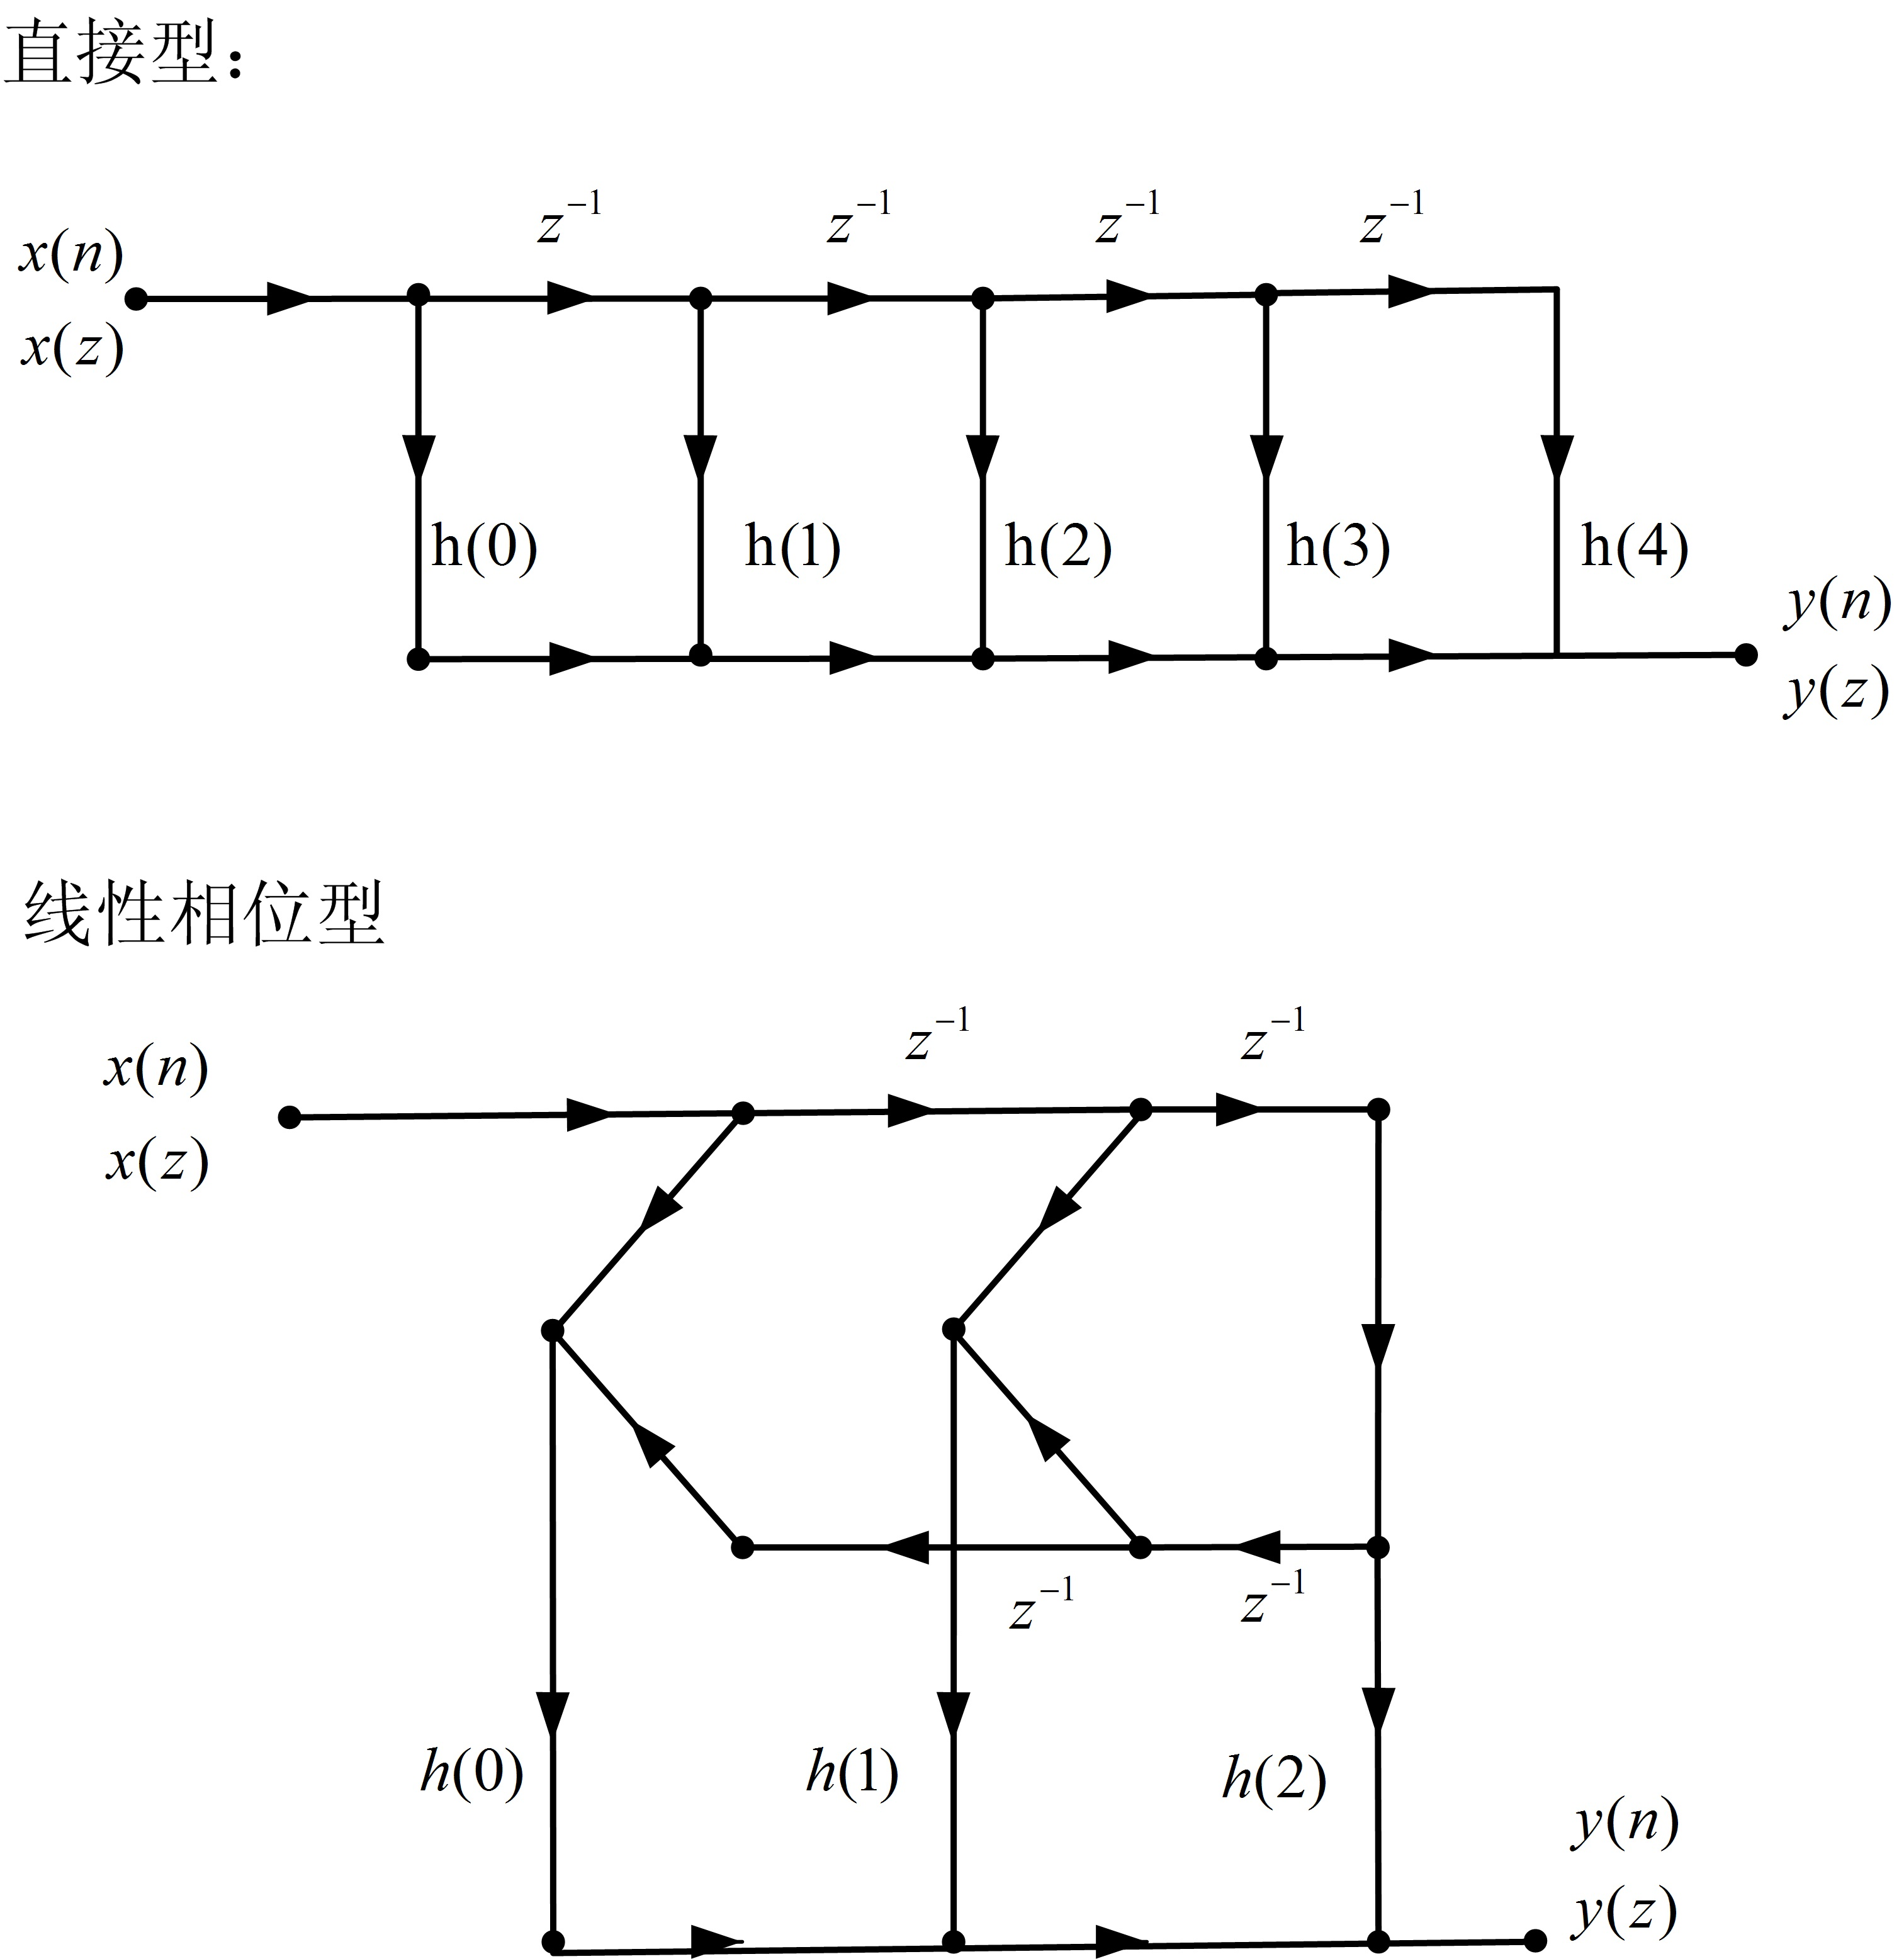
\includegraphics[width=0.6\textwidth]{example2.jpg}
          %\caption{该滤波器的网络结构}
      \end{figure}

\end{frame}
%%%%%%%%%%%%%%%%%%%%%%%%%%%%%%%%%%%%%%%%%%%%%%%%%%%%%%%%%%%%%%%%%%%%%%%%%%%%%%%%%%%%%%%%%%%%%%%

\section{频率采样法}
\subsection{频率域采样回顾}
%%%%%%%%%%%%%%%%%%%%%%%%%%%%%%%%%%%%%%%%%%%%%%%%%%%%%%%%%%%%%%%%%%%%%%%%%%%%%%%%%%%%%%%%%%%%%%
%\begin{frame}\frametitle{title}%[allowframebreaks][shrink]
%
%\end{frame}
%%%%%%%%%%%%%%%%%%%%%%%%%%%%%%%%%%%%%%%%%%%%%%%%%%%%%%%%%%%%%%%%%%%%%%%%%%%%%%%%%%%%%%%%%%%%%%%


%%%%%%%%%%%%%%%%%%%%%%%%%%%%%%%%%%%%%%%%%%%%%%%%%%%%%%%%%%%%%%%%%%%%%%%%%%%%%%%%%%%%%%%%%%%%%%
%\begin{frame}\frametitle{title}%[allowframebreaks][shrink]
%
%\end{frame}
%%%%%%%%%%%%%%%%%%%%%%%%%%%%%%%%%%%%%%%%%%%%%%%%%%%%%%%%%%%%%%%%%%%%%%%%%%%%%%%%%%%%%%%%%%%%%%%


%%%%%%%%%%%%%%%%%%%%%%%%%%%%%%%%%%%%%%%%%%%%%%%%%%%%%%%%%%%%%%%%%%%%%%%%%%%%%%%%%%%%%%%%%%%%%%
%\begin{frame}\frametitle{title}%[allowframebreaks][shrink]
%
%\end{frame}
%%%%%%%%%%%%%%%%%%%%%%%%%%%%%%%%%%%%%%%%%%%%%%%%%%%%%%%%%%%%%%%%%%%%%%%%%%%%%%%%%%%%%%%%%%%%%%%


%%%%%%%%%%%%%%%%%%%%%%%%%%%%%%%%%%%%%%%%%%%%%%%%%%%%%%%%%%%%%%%%%%%%%%%%%%%%%%%%%%%%%%%%%%%%%%
%\begin{frame}\frametitle{title}%[allowframebreaks][shrink]
%
%\end{frame}
%%%%%%%%%%%%%%%%%%%%%%%%%%%%%%%%%%%%%%%%%%%%%%%%%%%%%%%%%%%%%%%%%%%%%%%%%%%%%%%%%%%%%%%%%%%%%%%


%%%%%%%%%%%%%%%%%%%%%%%%%%%%%%%%%%%%%%%%%%%%%%%%%%%%%%%%%%%%%%%%%%%%%%%%%%%%%%%%%%%%%%%%%%%%%%
%\begin{frame}\frametitle{title}%[allowframebreaks][shrink]
%
%\end{frame}
%%%%%%%%%%%%%%%%%%%%%%%%%%%%%%%%%%%%%%%%%%%%%%%%%%%%%%%%%%%%%%%%%%%%%%%%%%%%%%%%%%%%%%%%%%%%%%%


%%%%%%%%%%%%%%%%%%%%%%%%%%%%%%%%%%%%%%%%%%%%%%%%%%%%%%%%%%%%%%%%%%%%%%%%%%%%%%%%%%%%%%%%%%%%%%
%\begin{frame}\frametitle{title}%[allowframebreaks][shrink]
%
%\end{frame}
%%%%%%%%%%%%%%%%%%%%%%%%%%%%%%%%%%%%%%%%%%%%%%%%%%%%%%%%%%%%%%%%%%%%%%%%%%%%%%%%%%%%%%%%%%%%%%%


%%%%%%%%%%%%%%%%%%%%%%%%%%%%%%%%%%%%%%%%%%%%%%%%%%%%%%%%%%%%%%%%%%%%%%%%%%%%%%%%%%%%%%%%%%%%%%
%\begin{frame}\frametitle{title}%[allowframebreaks][shrink]
%
%\end{frame}
%%%%%%%%%%%%%%%%%%%%%%%%%%%%%%%%%%%%%%%%%%%%%%%%%%%%%%%%%%%%%%%%%%%%%%%%%%%%%%%%%%%%%%%%%%%%%%%

\section{IIR和FIR数字滤波器的比较}
\subsection{频率域采样回顾}
%%%%%%%%%%%%%%%%%%%%%%%%%%%%%%%%%%%%%%%%%%%%%%%%%%%%%%%%%%%%%%%%%%%%%%%%%%%%%%%%%%%%%%%%%%%%%%
\begin{frame}\frametitle{提出问题}%[allowframebreaks][shrink]
\begin{wenti}
这两种滤波器各自有什么特点,在实际应用中应该如何去选择它们呢?
\end{wenti}
\end{frame}
%%%%%%%%%%%%%%%%%%%%%%%%%%%%%%%%%%%%%%%%%%%%%%%%%%%%%%%%%%%%%%%%%%%%%%%%%%%%%%%%%%%%%%%%%%%%%%%


%%%%%%%%%%%%%%%%%%%%%%%%%%%%%%%%%%%%%%%%%%%%%%%%%%%%%%%%%%%%%%%%%%%%%%%%%%%%%%%%%%%%%%%%%%%%%%
\begin{frame}\frametitle{从性能上来看}%[allowframebreaks][shrink]
\begin{enumerate}
  \item IIR滤波器的特点
            \begin{itemize}
              \item IIR滤波器系统函数的极点可位于单位圆内的任何地方,因此零点与极点相结合,可用较低的阶数获得较高的选择性,所用的存储单元少,计算量小,所以经济高效。
              \item 这个高效率是以相位的非线性为代价的。
            \end{itemize}
  \item FIR滤波器特点
            \begin{itemize}
              \item FIR数字滤波器可以得到严格的线性相位。
              \item 但FIR滤波器系统函数的极点固定在原点,而只能用较高的阶数达到高的选择性。对于同样的幅频特性指标,FIR滤波器所要求的阶数一般比IIR数字滤波器高5-10倍。使得成本较高,信号延时较大。
            \end{itemize}
  \item 综合考虑选择性和线性相位要求
            \begin{itemize}
              \item IIR滤波器必须加全通网络进行相位校正。从而大大增加滤波器的阶数和复杂性。
            \end{itemize}
  \end{enumerate}

\end{frame}
%%%%%%%%%%%%%%%%%%%%%%%%%%%%%%%%%%%%%%%%%%%%%%%%%%%%%%%%%%%%%%%%%%%%%%%%%%%%%%%%%%%%%%%%%%%%%%%


%%%%%%%%%%%%%%%%%%%%%%%%%%%%%%%%%%%%%%%%%%%%%%%%%%%%%%%%%%%%%%%%%%%%%%%%%%%%%%%%%%%%%%%%%%%%%%
\begin{frame}\frametitle{从结构上看}%[allowframebreaks][shrink]
\begin{enumerate}
  \item IIR滤波器的特点
      \begin{itemize}
        \item IIR滤波器必须采用递归结构,极点位置必须在单位圆内,否则系统不稳定。
        \item 这种结构中,由于运算过程中对序列的舍入处理得到的有限字长效应有时会引起寄生震荡。
      \end{itemize}
  \item FIR滤波器的特点
      \begin{itemize}
        \item FIR滤波器主要采用非递归结构,不存在稳定性问题。
        \item FIR滤波器可以采用FFT算法实现,在相同阶数的情况下,运算速度可以大大提高。
      \end{itemize}
\end{enumerate}
\end{frame}
%%%%%%%%%%%%%%%%%%%%%%%%%%%%%%%%%%%%%%%%%%%%%%%%%%%%%%%%%%%%%%%%%%%%%%%%%%%%%%%%%%%%%%%%%%%%%%%


%%%%%%%%%%%%%%%%%%%%%%%%%%%%%%%%%%%%%%%%%%%%%%%%%%%%%%%%%%%%%%%%%%%%%%%%%%%%%%%%%%%%%%%%%%%%%%
\begin{frame}\frametitle{从设计工具上看}%[allowframebreaks][shrink]

\end{frame}
%%%%%%%%%%%%%%%%%%%%%%%%%%%%%%%%%%%%%%%%%%%%%%%%%%%%%%%%%%%%%%%%%%%%%%%%%%%%%%%%%%%%%%%%%%%%%%%


\end{document}

